\documentclass[11pt,a4]{article} 
\usepackage[ansinew]{inputenc} %Schrifttyp und Umlaute
\usepackage{epsfig} %Nutzung von eps files
%\usepackage[dvips]{epsfig} %Nutzung von eps files
%\usepackage[final]{graphicx}    
%\usepackage[off]{auto-pst-pdf}     % necessary for psfrag to work
\usepackage{epstopdf} 

\usepackage[bf,sf,compact]{titlesec} 
\usepackage{fancyhdr} 
\usepackage{amsmath}
\usepackage{amssymb} %Symbole nach AMS
\usepackage{amstext}
\usepackage{theorem}
\usepackage{subfigure}
\usepackage{booktabs}

\usepackage{flafter}
\usepackage{exscale}
\usepackage{float}   % for minipages
\usepackage{psfrag}
\usepackage{listings}
\usepackage{color} %red, green, blue, yellow, cyan, magenta, black, white

\setlength{\parindent}{0cm} 
\setlength{\textwidth}{16cm}
\setlength{\oddsidemargin}{0cm}  
\setlength{\voffset}{-2,8cm}  
\setlength{\textheight}{25cm} 
\setlength{\arrayrulewidth}{0,3mm} 
\setlength{\textheight}{25cm} 

\renewcommand{\labelenumi}{\alph{enumi})} 
\sloppy
\usepackage{xcolor}

% Linkcolour
\usepackage[	 
	colorlinks=true,
 	breaklinks=true,
	citecolor=black,
	linkcolor=black,	
	menucolor=black,	
	urlcolor=blue
]{hyperref}

\definecolor{mygreen}{RGB}{28,172,0} % color values Red, Green, Blue
\definecolor{mylilas}{RGB}{170,55,241}

\lstset{language=Matlab,%
    %basicstyle=\color{red},
    breaklines=true,%
    morekeywords={matlab2tikz},
    keywordstyle=\color{blue},%
    morekeywords=[2]{1}, keywordstyle=[2]{\color{black}},
    identifierstyle=\color{black},%
    stringstyle=\color{mylilas},
    commentstyle=\color{mygreen},%
    showstringspaces=false,%without this there will be a symbol in the places where there is a space
    numbers=left,%
    numberstyle={\tiny \color{black}},% size of the numbers
    numbersep=9pt, % this defines how far the numbers are from the text   
}


\begin{document} %hier geht es los

\thispagestyle{empty} 
\begin{tabular*}{16cm}{lr} \hline \\ %Tabelle mit zwei Spalten, in jeder Spalte eine minipage, neue Zeile mit \\
    \begin{minipage}{10cm} %Anfang minipage in linker Spalte, Breite 8cm
            \textsf{Technische Universit\"at Dortmund \\ %Schriftgröße smallface
            Department of Biochemical and Chemical Engineering \\
            Chair of Process Dynamics and Operations \\
            Prof.~Dr.~Sebastian Engell \\}
    \end{minipage} & %Ende minipage in linker Spalte
    \begin{minipage}{6cm} %Anfang minipage in rechter Spalte, Breite 8cm
            \setlength{\unitlength}{1cm} %Formatierung, Platzierung und Einfuegen des ASTLOGOS
            \begin{picture}(8,1) 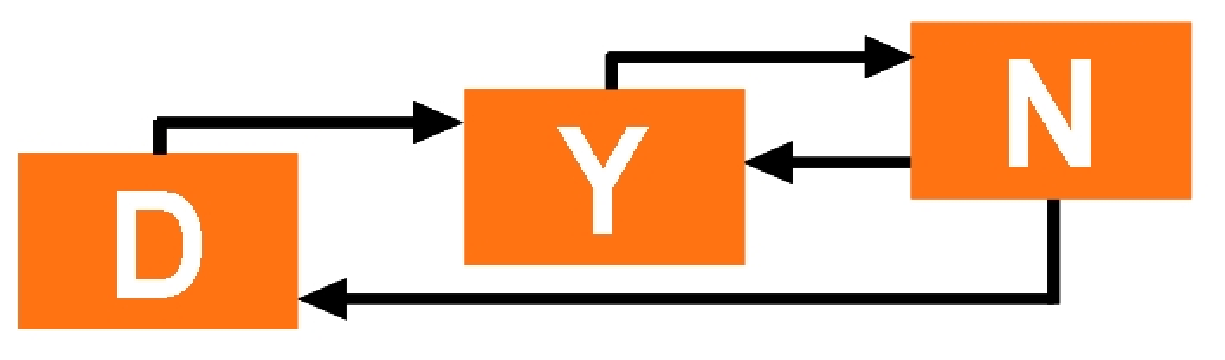
\epsfig{file= Astlogo.eps, width=5cm}
            \end{picture}\par
    \end{minipage} \\ \hline %Ende minipage in rechter Spalte
\end{tabular*} %Ende Tabelle




\vspace{5cm}

\begin{center} 

\LARGE{\bfseries DEVELOPMENT OF LOCAL POSITIONING SYSTEM FOR A PIPE-LESS PLANT\\

\vspace{0.25cm}
    Automation \& Robotics 
    
    Group Project SS18 \\}
    
\vspace{3cm}
\emph{Group Members:}\\[0.2cm]
Abdulrahman Abouelkhair(4511328)\\	                                         % Author info
Medhini Rajagopal Balamurugan(4511328)\\
Stefan Rottstegge(4511328)\\
Stephan Vette(4511328)\\[1.5cm]

\emph{Supervisors:}\\[0.2cm]
Afaq Ahmad \\ 
Marina Rantanen-Mod\'eer\\[1.5cm]	                                     % Supervisor info
\end{center}



%%%%%%%%%%%%%%%%%%%%%%%%%%%% ABSTRACT
\clearpage
\titleformat{\section}{\Large\bf}{\thesection:}{20pt}{}
\setcounter{enumi}{0} \section*{Abstract} %

\subsection*{Introduction}
The pipe-less plant at the Process Dynamics and Operations group is an experimental setup of Automated Guided Vehicles (AGVs) moving between various stations. The AGVs dynamically change trajectories in operational mode based on a Model Predicative Control (MPC) scheme with the objective to get from one station to the other while at the same time avoiding each other. The current positioning system is based on pattern recognition where the system tracks each AGV based on a unique pattern of LEDs via a camera that overlooks the plant. 
\subsection*{Motivation for new positioning system
}
The vision based positioning system displays some flaws and should be replaced by a system more adapted to the actual operational environment of the experimental plant. The following problems have been identified in the current setup of the system: 

\begin{itemize}
	\item No position feedback in bright day-light conditions 
	\item A ``\textit{fish-eye camera lense problem}'', meaning that the position error grows with the distance from the center of the image caused by the distortion a wide angle lense creates
	\item Problems related to the software implementation restricting the usage of incoming information from the camera
\end{itemize}

\subsection*{Project objective
}
The project aimed at first evaluating different potential positioning systems, selecting one of them based on defined metrics and then to develop a proof-of-concept based on the chosen technology for the experimental pipe-less production plant in a model driven fashion. After going through four different alternatives including a triangulation based methods for indoor applications, another pattern recognition based method (such as QR-codes), map-based localization, and Radio-Frequency Identification (RFID), the latter was chosen for further evaluation and implementation.
\subsection*{Theoretical Background}
RFID is a versatile technology with multiple application areas, e.g. access control, race tracking and positioning. Automated multi-agent systems are increasingly utilizing RFID for localization as the technology has been proven to have many advantages over vision based positioning systems.It uses electromagnetic fields to automatically identify and track tags attached to objects. There are two potential ways to implement an RFID localization system. One option is based on active RFID transmitters and reader with wide coverage areas that can be placed along the edges of the plant area and on each AGV. The other option is based on comparatively many passive tags, uniformly placed, on the ground of the plant area and active readers on the AGVs. The latter option was chosen for the project based on cost efficiency, system scalability and from literature proven applicability.
\subsection*{Hardware
}
An RFID system is made up of two parts: a tag and a reader. RFID tags are embedded with a transmitter and a receiver. The RFID component on the tags has two parts: a microchip that stores and processes information, and an antenna to receive and transmit a signal, which partly contains the unique ID of the tag. The hardware components which are added to the AGVs comprise an RFID antenna, an RFID reader and a WiFi module. All the devices are supplied with 5V. The antenna is connected to the reader via a coaxial so called ``\textit{SubMiniature version A}''(SMA) cable and the reader communicates via an RX/TX interface. The RFID reader and the WiFi-module are connected via wired serial communication. The WiFi module then transmits the reader data through the local network, using TCP/IP communication. The system data is lastly received by a PC that represents the control hub of the plant through a framework implemented in C Sharp (C\#). 
\subsection*{Communication
}
The WiFi-Module is connected to the same router as the PC on which the system user interface is running. A TCP-Client was established in the C\# framework in order to handle incoming RFID data. The WiFi-module continuously sends data and the algorithm calculating AGV position prompts for this data as position and/or orientation of an AGV needs to be computed.
\subsection*{Localization
}
The implemented positioning algorithm requires the ID and the received signal strength indication (RSSI) of at least three RFID tags to calculate the position of the antenna. The RSSI gives a relation between the detected tag and the distance to it, in other words, a radius. The system has a record of the position of each tag and the ID of each tag hence holds information about the uniquely defined position of the tag. With three positions and the three corresponding radii, one can use trilateration to compute the position of the antenna.  
\subsection*{Initialization Procedure
}
Initially the system cannot  know the orientation of the AGV even if it can read enough RFID tags, as the tags only provide the x and y coordinates of the antenna itself (which is located off center on the robot). The main goal of the initializing procedure is to estimate both the starting position and orientation. During the turn, the robot will make a short stop every 45° and estimate the position of the antenna at that point. At the end of the procedure, the algorithm calculates the center of the eight recorded points. It takes two positions plus their corresponding positions at the other side (plus 180$^{\circ}$) and computes the intersection of the linear function which goes through the position and its corresponding point. To estimate the orientation the algorithm computes the angle between the estimated position and the position of the antenna at 360$^{\circ}$/0$^{\circ}$. 
\subsection*{Demonstrator and results}
A proof-of-concept for an RFID based localization system has been built in a model-driven fashion. The new system was simulated using Matlab to evaluate its applicability and overcome engineering problems at an early stage of the design phase. An initialization algorithm has been designed and implemented to calculate the starting position and heading of the robot.  Simulations show an average position error of 0.5 cm. Analogously, the orientation of an error of around 10$^{\circ}$. The system prototype consists of a reader and an area of nine tags (3x3).  The measured position error in the experimental setup was on average 2.5 cm. The error of the orientation was on average about 23$^{\circ}$. This significant difference to simulated results was caused by two main reasons: Firstly, some tags could not be detected by the reader. Secondly, the test board was quite small as it consisted of so few RFID tags which meant that it was not representative enough of the intended design. To summarize, it can be said that on the one hand a rather low-cost, scalable solution was designed which can work in any area independent for any light conditions.  On the other hand, the accuracy of the technology is not very reliable according to the experiments made. This can be improved in further work with a better system setup and an improved localizing algorithm.



%%%%%%%%%%%%%%%%%%%%%%%%%%%%
\clearpage
\tableofcontents

\newpage
\listoffigures
\listoftables


\setlength{\textheight}{20cm}

\pagestyle{fancy} 
\lhead{Final report, TITLE, \today}
\chead{}
\rhead{Page \thepage}
\lfoot{}
\cfoot{}
\rfoot{} 
\renewcommand{\headrulewidth}{0.4pt} 

\setlength{\topmargin}{2cm} %oberer Rand bis Oberkante Kopfzeile

\makeatletter \def\usecounter#1{\@nmbrlisttrue\def\@listctr{#1}}
\makeatother 
\setcounter{figure}{0}
\setcounter{table}{0} 



%Introduction
\titleformat{\section}{\Large\bf}{\thesection}{20pt}{}
\section{Introduction}

In today\textquoteright s world, the development and implementation of the positioning system for the autonomous vehicle in a confined space remains to be a major issue and hindrance to a better control system. Though there exists many types of local positioning systems, the precision remains to be still a challenge. This problem becomes critical in a place of no GPS access.
This project aims at investigating various methods of indoor localization and to develop a proof-of-concept for the existing pipeless plant setup. \\

In the past years students and researchers at the Process Dynamics and Operations group at the TU Dortmund have developed this plant with vision based positioning system which need to be replaced to improve the overall efficiency of the system. Both the old and newly implemented techniques are written in C\# that sends the position update to the Python based controller code.\\

In this project, various potential positioning techniques were discussed and their pros and cons were compared. The different localization methods would be further discussed in section \ref{Sec_selectionp}.After a thorough four different alternatives including a triangulation based methods for indoor applications, another pattern recognition based method (such as QR-codes), map-based localization, \textit{Radio Frequency Identification} was chosen to be the ideal technique. It is a versatile technology with multiple application areas, e.g. access control, race tracking and positioning. Automated multi-agent systems are increasingly utilizing RFID for localization as the technology has been proven to have many advantages over vision based positioning systems \ref{Sec_theor}.There are two potential ways to implement an RFID localization system namely active and passive. The latter is based on comparatively many passive tags, uniformly placed, on the ground of the plant area and active readers on the AGVs. The latter option was chosen for the project based on cost efficiency, system scalability and from literature proven applicability. \\

An RFID system is made up of two parts: a tag and a reader. RFID tags are embedded with a transmitter and a receiver. The RFID component on the tags has two parts: a microchip that stores and processes information, and an antenna to receive and transmit a signal, which partly contains the unique ID of the tag. The hardware components which are added to the AGVs comprise an RFID antenna, an RFID reader and a WiFi module. Further hardware implementation is explained in section \ref{Sec_Imp}. The WiFi module then transmits the reader data through the local network, using TCP/IP communication. The system data is lastly received by a PC that represents the control hub of the plant through a framework implemented in C Sharp (\texttt{C\#}). A TCP-Client was established in the \texttt{C\#} framework in order to handle incoming RFID data. The WiFi-module continuously sends data and the algorithm calculating AGV position prompts for this data as position and/or orientation of an AGV needs to be computed.\\

The implemented positioning algorithm requires the ID and the received signal strength indication (RSSI) of at least three RFID tags to calculate the position of the antenna. The RSSI gives a relation between the detected tag and the distance to it, in other words, a radius. The system has a record of the position of each tag and the ID of each tag hence holds information about the uniquely defined position of the tag. With three positions and the three corresponding radii, one can use trilateration to compute the position of the antenna. This concept was developed into simulation which would be discussed in section \ref{Sec_Sim}. The experiment bbbased results will be explained in \ref{Sec_Imp}. Based on the experiment, conclusion and future work are given in section \ref{Sec_Conc} and \ref{Sec_fut} respectively.







%Theory
\clearpage
\titleformat{\section}{\Large\bf}{\thesection}{20pt}{}
\section{Pipeless Plant} %

\subsection{Existing setup}

\subsection{Problems with the Existing Setup}
..

zb
\begin{itemize}
\item Fish eye
\item Sunlight..
\end{itemize}

%%%%%%%%%%%%%%%%%%%%%%%%%%%%
\titleformat{\section}{\Large\bf}{\thesection}{20pt}{}
\section{Selection Process} \label{Sec_selectionp}

Since the main aim of the project is to improve the positioning system of the existing setup, several  other techniques were discussed, ending up in four methods namely ``\textit{triangulation}'',``\textit{pattern recognition}'',``\textit{radio frequency identification}'', ``\textit{map-based localization}''. The pros and cons were listed and the mentioned techniques were compared. The following section deals with a brief description of the above mentioned techniques.\\

\subsection{Triangulation} %stefan
Since the plant has a specified size in which the location of multiple objects has to be performed the method of triangulation is one promising technic in which research was made. 
Triangulation was already a common principle of measurement in the 18th century and it is divided into active and passive triangulation. Passive triangulation is a geometrical method based on two measurement stations which positions are known exactly. At these two measurement points angels of the desired point in space are measured to compute the localization in the specified coordinate system (x, y, z) with trigonometrical formulas.
With respect to the system setup used in the 18th century nowadays two cameras are installed to perform a geographical method of 3D object-data estimation as shown in fig. \ref{Triangulation} \cite{Prinzip3DVideometrie.}.
\begin{figure}[!htbp]
\centering
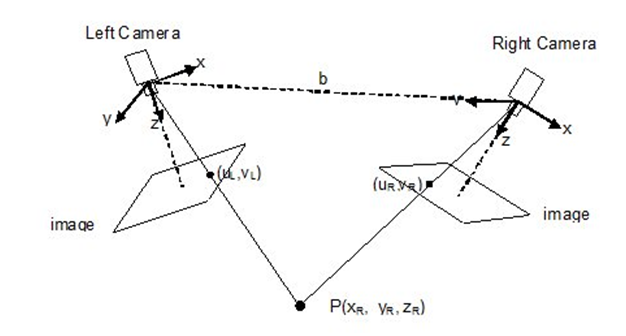
\includegraphics[width = 16cm]{Pictures/Triangulation}
\caption{Passive triangulation setup with two cameras [3]}
\label{Triangulation}
\end{figure}\\
To solve the problem of position estimation, it is necessary to know the parameters of the left and the right camera visualized in the figure. In theory the triangulation is trivial, since each and every point of the images of the respective cameras maps to a line in 3D space. If a pair of corresponding points, in the case of the pipesless plant it would be an AGV is found, the projection of a point x in 3D space can be computed. 
Active triangulation in comparison to passive triangulation needs one camera and at least one source of structured light (e.g. Laser). The geometrical location and orientation of the camera and light source in space need to be known. Two possible setups with either a laser point or a stripe as structured light are shown in fig. \ref{ative_Triangulation} \cite{MultiObjectTriangulation.}\cite{laser_triangulation}.
\begin{figure}[!htbp]
\centering
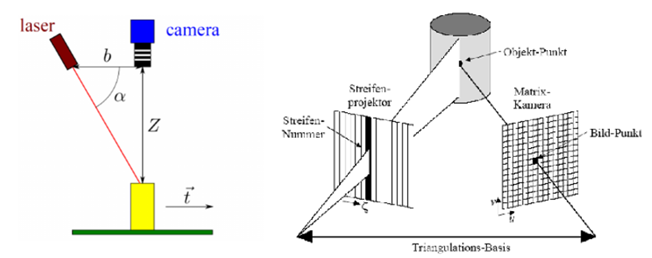
\includegraphics[width = 16cm]{Pictures/acticetriangulation}
\caption{Active triangulation}
\label{ative_Triangulation}
\end{figure}\\
To solve the active triangulation problem, the structured light has to point an object which location is desired to estimate. If this point is found on the 2D image of the camera, a triangulation with basic trigonometrical formulas which are using the properties and parameters of the camera and light source can be performed and the position of the AGV can be estimated. 
\pagebreak
\subsubsection*{Implementation} 
One possible way to implement a solution for the passive triangulation is to attach 2 high resolution cameras with USB 3.0 on two edges of the plant as shown in fig. \ref{ativeTriangulationimplementation}.\\
\begin{figure}[!htbp]
	\centering
	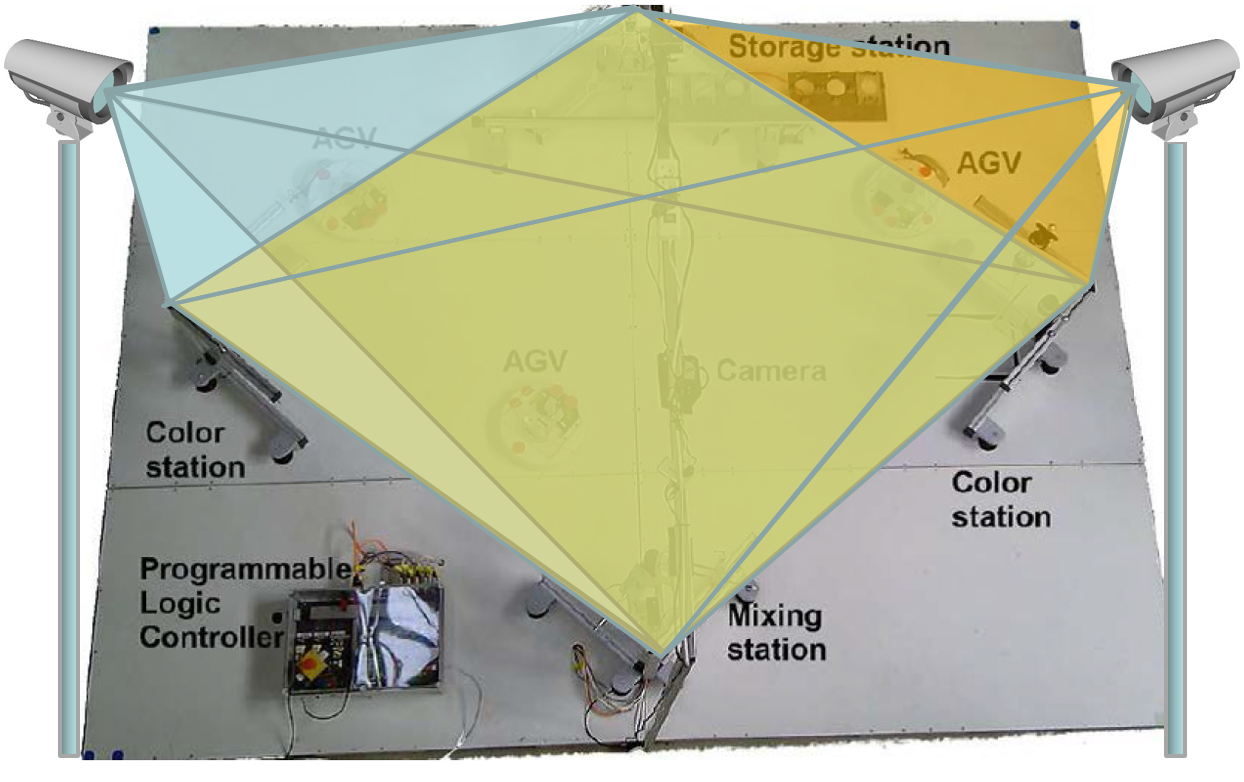
\includegraphics[width = 16cm]{Pictures/triangulationimplementatio}
	\caption{Implementation of passive triangulation}
	\label{ativeTriangulationimplementation}
\end{figure}\\%
The left and right camera are sequentially taking pictures which are transmitted to the plants computer where the image processing takes place.\\ 
\pagebreak
Based on the research made , two tables with advantages and disadvantages of the two triangulation systems are created.
\begin{table}[!htbp]
\centering
\begin{tabular}{|l|l|}
\hline
\multicolumn{2}{|c|}{\textbf{Passive Triangulation}}                                                                                                                  \\ \hline
\multicolumn{1}{|c|}{\textbf{Pro}}                                                                                    & \multicolumn{1}{c|}{\textbf{Con}}   \\ \hline
Upgrade to USB 3.0 for faster data transmitting possible                                                                   & Light dependent                          \\ \hline
\begin{tabular}[c]{@{}l@{}}Upgrade to a camera with higher resolution to reduce \\ measurement error possible\end{tabular} & New concept of orientation may be needed \\ \hline
No Fish-Eye-Lense problem                                                                                                  & Limited range of observation             \\ \hline
Low cost                                                                                                                   &                                          \\ \hline
\end{tabular}
\caption{Pros and cons points of passive triangulation}
\label{pro_con_passive_tri}
\end{table}
\begin{table}[!htbp]
\centering
\begin{tabular}{|l|l|}
\hline
\multicolumn{2}{|c|}{\textbf{Active Triangulation}}                                                                                                                     \\ \hline
\multicolumn{1}{|c|}{\textbf{Pro}}                                                                                    & \multicolumn{1}{c|}{\textbf{Con}}     \\ \hline
Upgrade to USB 3.0 for faster data transmitting possible                                                                   & New unknown laser technology is needed     \\ \hline
\begin{tabular}[c]{@{}l@{}}Upgrade to a camera with higher resolution to reduce \\ measurement error possible\end{tabular} & High costs for several lasers (one per AGV) \\ \hline
Easy detection of laser points on camera image                                                                             & Laser needs to move while AGVs are moving  \\ \hline
                                                                                                                           & Limited range of observation               \\ \hline
                                                                                                                           & Light dependent                            \\ \hline
\end{tabular}
\caption{Pros and cons points of active triangulation}
\label{pro_con_active_tri}
\end{table}
\pagebreak
\subsection{Pattern Recognition} %medhini
\subsubsection*{Summary}
In this type of localization, estimation of the robot is done in indoor environments using
only on-board sensors, namely a web-cam and a compass. The ceiling of the plant is constructed with a pattern of static landmarks whose positions are known a priori. All landmarks are indistinguishable against each other and might additionally be distributed along the ceiling in a periodic pattern. The landmark attached to the ceiling can be lights, QR codes, sensors or other
reference points. The ceiling is used, since it is immune to changes. A camera is installed on the robot, which takes snapshots of the ceiling. The robot pose relative to the landmark is  calculated with the help of the distance of the landmark to the center of the image and its angle relatively to the direction of the  robot motion. An IMU device is additionally used to give the absolute orientation of the robot in the plant. The Markov Localization (ML) algorithm is used to estimate
the belief grid of the robot position inside the environment. 

\begin{figure}[!htbp]
	\centering
	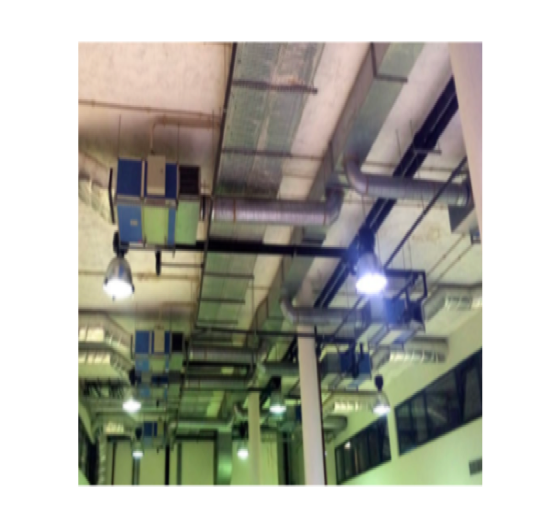
\includegraphics[width = 10cm]{Pictures/PR.png}
	\caption{Ceiling with periodic patterns of lamps acting as landmarks. }
	\label{Pattern Recognition}
\end{figure}
\subsubsection*{Implementation}
The goal is to compute the pose of a mobile robot inside an indoor environment using a camera and an IMU device. As mentioned, Markov Localization is used to create a belief grid of the robot in the plant environment. This is done with the help of the snapshots of the ceiling taken by the camera. As seen in the figure \ref{PatternRecognition1}, the blue and black areas have lower belief and green and yellow areas have higher belief. The obtained pattern is evaluated and based on the pattern, the position of the robot is estimated. Thus with the help of the camera and the IMU device, both the position and orientation is obtained. 


\begin{figure}[!htbp]
	\centering
	\begin{minipage}{.5\textwidth}
		\centering
		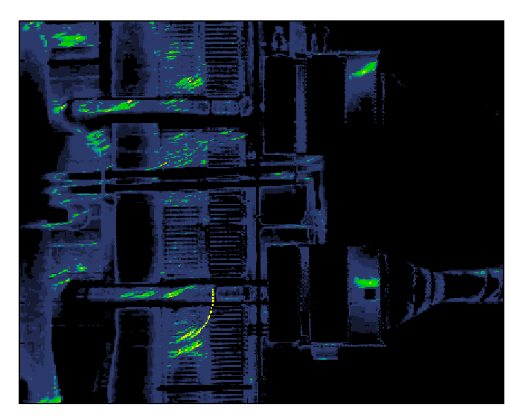
\includegraphics[width = 7cm]{Pictures/beliefgrid.png}
		\caption{Belief grid of the robot in the plant}
		\label{PatternRecognition1}
	\end{minipage}%
	\begin{minipage}{.5\textwidth}
		\centering
		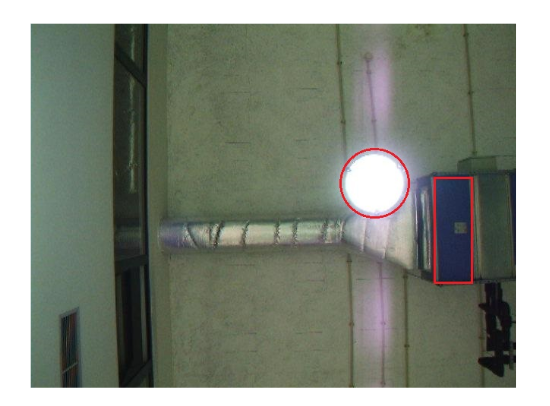
\includegraphics[width = 8cm]{Pictures/snapshot.png}
		\caption{Snapshot of the ceiling }
		\label{PatternRecognition2}
	\end{minipage}
\end{figure}

\subsubsection*{Pro and con}
Based on the research,the advantages and disadvantages of Mobile Robot Localization based on Pattern Recognition are created.
\begin{table}[!htbp]
	\centering
	\begin{tabular}{|l|l|}
		\hline
		
		\multicolumn{1}{|c|}{\textbf{Pro}}                                                                                    & \multicolumn{1}{c|}{\textbf{Con}}   \\ \hline
		\begin{tabular}[c]{@{}l@{}}The ceiling is usually immune to changes                                                                  
			as a  \\ reference and implement  landmarks
			on the ceiling itself  \end{tabular}                                                & \begin{tabular}[c]{@{}l@{}}Complex and many changes have to be \\ added to the plant   \end{tabular}                                    \\ \hline
		
		
		No Fish-Eye-Lense problem                                                                                            & Cost intensive                                 \\ \hline
		& Light dependent                            \\ \hline
		
	\end{tabular}
	\caption{Pros and cons points of Mobile Robot Localization based on Pattern Recognition
	}
	\label{pro_con_Mobile Robot Localization based on Pattern Recognition
	}
\end{table}
\pagebreak

\subsection[RFID]{RFID\footnote{Stephan}} % stephan around 2 pages
\subsubsection*{Summary} 
One of the possible solutions to solve the challenging problem of indoor localization is the use of the Radio-frequency Identification (RFID) technology. The main areas of this technology is indeed still supply chains, transport, manufacturing, personnel access, animal tagging, toll collection \cite{Bai_overviewof},  but also has become popular in localizing objects and persons. Where in the main applications only the identification has to be realized, also the strength of the signals is important to estimate the position of a certain object.\\
The main idea of those systems is that a reader detects a tag and reads its information. The technology can be divided into three main types: passive, semi-passive and active systems. A passive system, like it is been shown in fig. \ref{RFID_Passive}, consists of a reader, which is connected to an antenna and a computer and a passive tag.\\
\begin{figure}[!htbp]
\centering
\begin{minipage}{.5\textwidth}
\centering
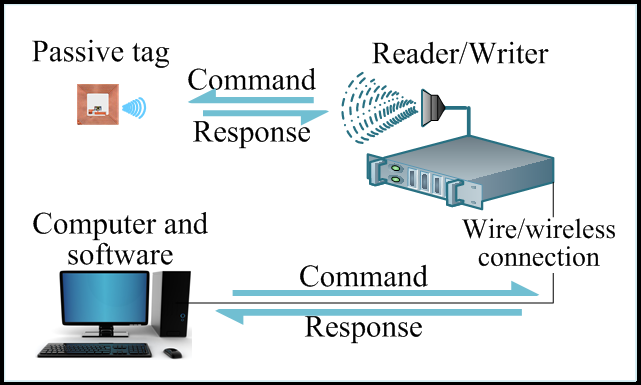
\includegraphics[width = 7cm]{Pictures/RFID_Passive}%
\caption{Passive RFID System}
\label{RFID_Passive}
\end{minipage}%
\begin{minipage}{.5\textwidth}
\centering
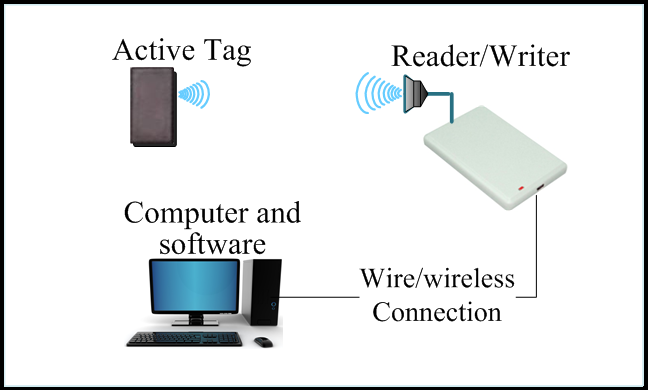
\includegraphics[width = 7cm]{Pictures/RFID_Active}%
\caption{Active RFID System}
\label{RFID_Active}
\end{minipage}
\end{figure}\\
The system is called passive, because the power supply is realized by the radio signal of the reader. In case where the tag is in the reading range of the reader, the tags gets enough power to send predefined information (for example ID) back. The active system (see fig.\ref{RFID_Active}) in comparison has an active tag which has an own power supply. The semi-passive tag has a battery build in that the tag has more power to communicate, but is not used to generate radio frequency signals.\\ 
Another classification of RFID systems is the frequency of the radio waves. It can reach from 0.135 MHz (Low Frequency) to 5875 MHz (Super High Frequency). The table \ref{RFID_Systems} gives an overview about the systems related to reading ranges, reading rates and the ability to read near metal or water.\\
\begin{table}[!htbp]
\centering
\begin{tabular}{c}
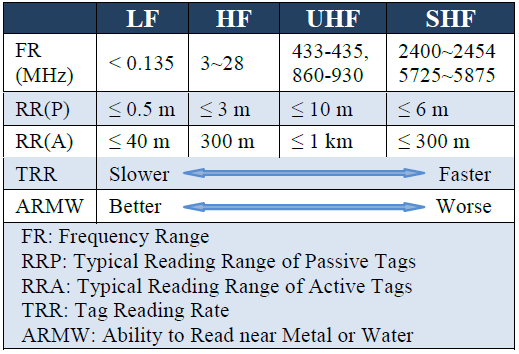
\includegraphics[width = 9cm]{Pictures/RFID_Systems}
\end{tabular}
\caption{Overview RFID systems}
\label{RFID_Systems}
\end{table}\\
It can be seen that the passive systems in general have a smaller reading range then the active systems and has a bigger data rate. But it has also to be take into account, that passive tags are cheaper then active tags.   
\subsubsection*{Implementation}
There are mainly two different ways to realize a localization system of the AGVs in the pipeless plant. Based on the fact that the plant has a size of 3 by 4 meter, the tracking can be carried out with a passive system in which a couple of passive tags on the floor can be used as landmarks. In this case the reader plus the antenna would be placed on the AGV and localize with the help of the detected tags. The other systems consists of three or four reader in each corner of the plant and an active tag on each AGV.
\pagebreak
\subsubsection*{Pro and con}
Based on the research made, two tables with advantages and disadvantages of the two RFID systems are created.\\ 
\begin{table}[!htbp]
\centering
\begin{tabular}{|l|l|}
\hline
\multicolumn{2}{|c|}{\textbf{Active RFID system}}                                                                                                                                                                                \\ \hline
\multicolumn{1}{|c|}{\textbf{Pro}}                                                                                & \multicolumn{1}{c|}{\textbf{Con}}                                                                            \\ \hline
Light independent                                                                                                 & Prototype more expansive (3 reader + avtive tags)                                                            \\ \hline
Space unlimited                                                                                                   & \begin{tabular}[c]{@{}l@{}}Datarate is related to the amount of\\ detected tags a the same time\end{tabular} \\ \hline
\begin{tabular}[c]{@{}l@{}}Localization only has to be realized in\\ a bigger area - medium accuracy\end{tabular} & \begin{tabular}[c]{@{}l@{}}Anticollision need, cause more AGVs are\\ used at the same time\end{tabular}      \\ \hline
\begin{tabular}[c]{@{}l@{}}Wired communication between reader and \\ computer possible\end{tabular}               & \begin{tabular}[c]{@{}l@{}}Signal strength can be influenced by envirnonment\\ (metal or water)\end{tabular} \\ \hline
Simple algorithm (Trilateration)                                                                                  &                                                                                                              \\ \hline
\end{tabular}
\caption{Pro and cons of active RFID system}
\label{my-label}
\end{table}
\begin{table}[!htbp]
\centering
\begin{tabular}{|l|l|}
\hline
\multicolumn{2}{|c|}{\textbf{Passive RFID system}}                                                                                                                                                                                            \\ \hline
\multicolumn{1}{|c|}{\textbf{Pro}}                                                                                             & \multicolumn{1}{c|}{\textbf{Con}}                                                                            \\ \hline
Light independent                                                                                                               & \begin{tabular}[c]{@{}l@{}}Communication between AGV and computer \\ has to be realized\end{tabular}         \\ \hline
Space unlimited                                                                                                                & \begin{tabular}[c]{@{}l@{}}Data rate is related to the amount of\\ detected tags a the same time\end{tabular} \\ \hline
\begin{tabular}[c]{@{}l@{}}Localization only has to be realized between\\ four tags (small area) - high accuracy\end{tabular} & \begin{tabular}[c]{@{}l@{}}Anticollision need, cause more tags are\\ detected at the same time\end{tabular}  \\ \hline
Simple algorithm (Trilateration)                                                                                               &                                                                                                              \\ \hline
Prototype cheap (1 reader + passive tags)                                                                                      &                                                                                                              \\ \hline
\end{tabular}
\caption{Pro and cons passive RFID system}
\label{Pro and Cons of the passive RFID system}
\end{table}
\pagebreak
\subsection{Map-Based Localization\cite{mbl}} %abdul
\subsubsection*{Summary}
AMCL (Adaptive Monte Carlo Localization) is a probabilistic localization system for a robot moving in 2D. It implements the adaptive (or KLD-sampling) Monte Carlo localization\cite{acml1}\cite{acml2} approach, which uses a particle filter to track the pose of a robot against a known map.
\begin{figure}[!htbp]
	\centering
	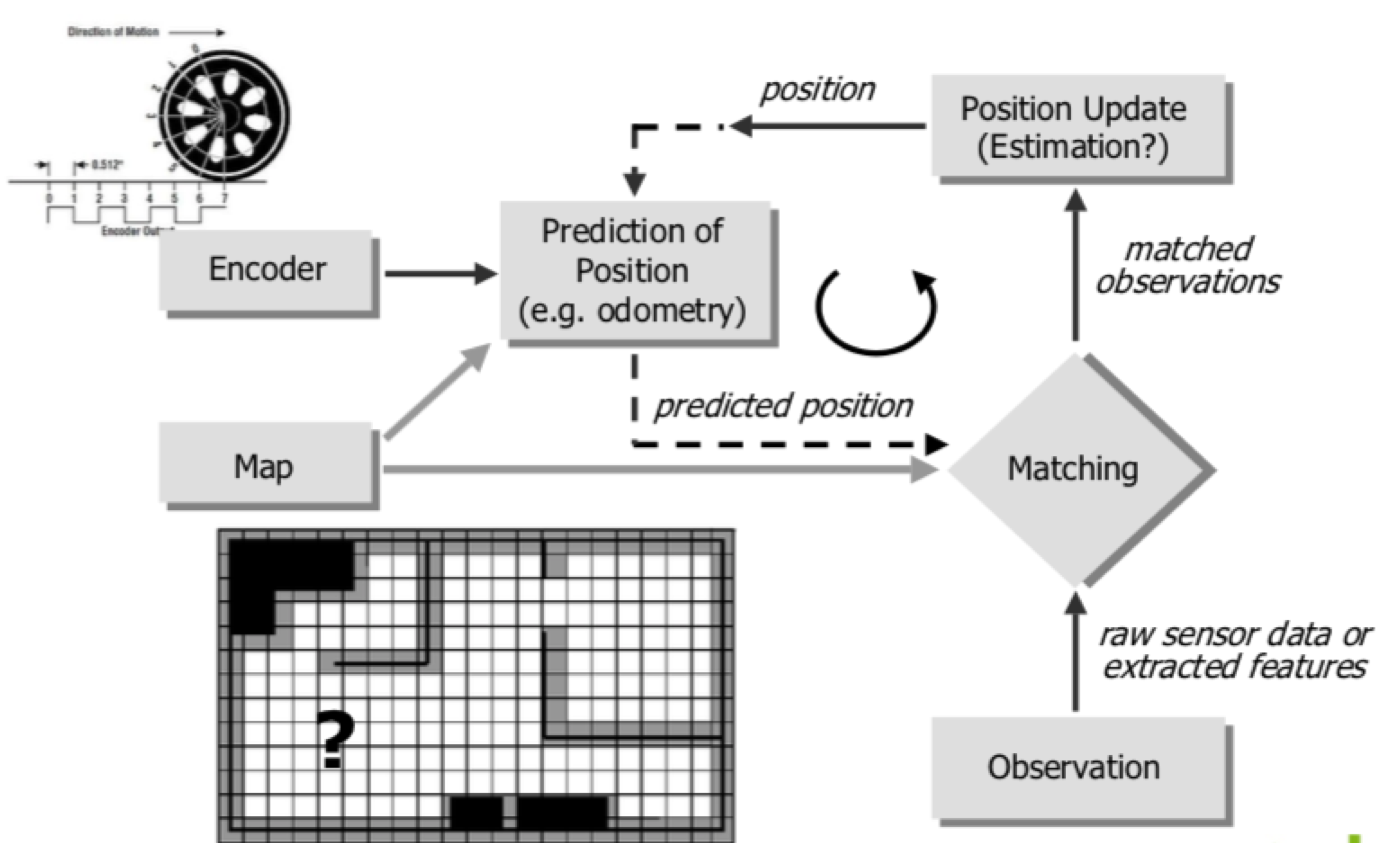
\includegraphics[width = 15cm]{Pictures/amcl}
	\caption{Adaptive Monte Carlo localization}
	\label{amcl}
\end{figure}\\
amcl takes in a laser-based map, laser scans, and Odom scan, and outputs pose estimates (see fig.\ref{amcl}). On startup, amcl initializes its particle filter according to the parameters provided. Note that, because of the defaults, if no parameters are set, the initial filter state will be a moderately sized particle cloud centered about (0,0,0).
\\
\subsubsection*{Implementation}
To implement such a technique a global and local map should be created as shown in fig. \ref{global_map} and fig. \ref{local_map}.
\begin{figure}[!htbp]
	\centering
	\begin{minipage}{.5\textwidth}
		\centering
		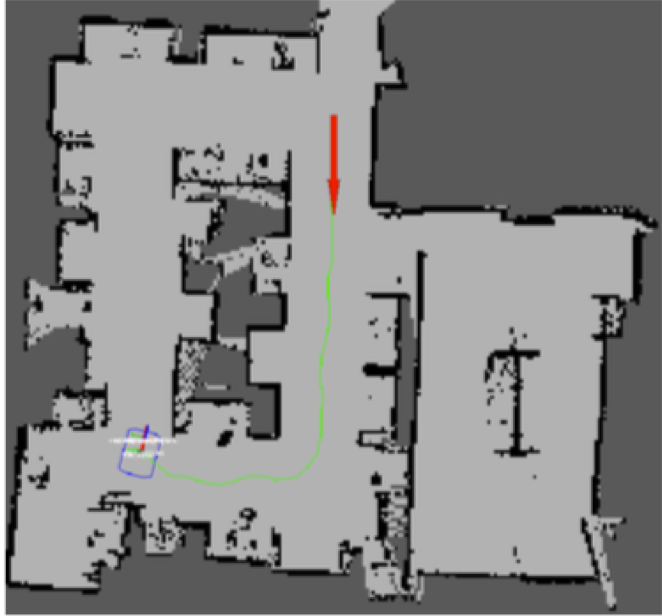
\includegraphics[width = 6cm]{Pictures/global}%
		\caption{Global Map}
		\label{global_map}
	\end{minipage}%
	\begin{minipage}{.5\textwidth}
		\centering
		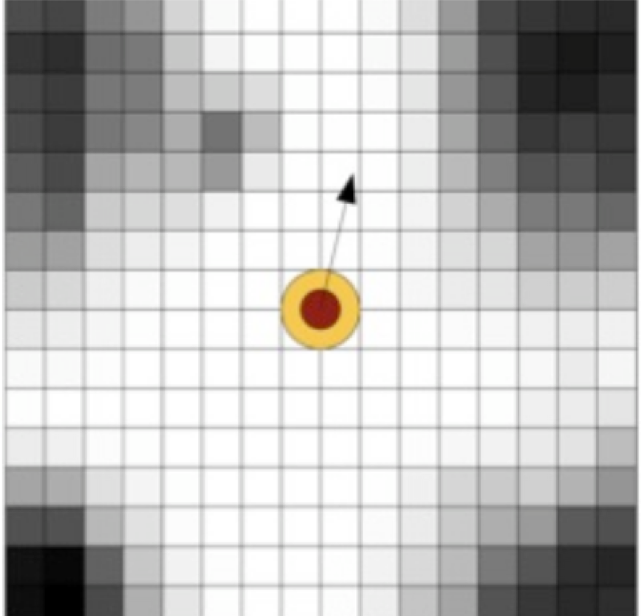
\includegraphics[width = 6cm]{Pictures/local}%
		\caption{Local Map}
		\label{local_map}
	\end{minipage}
\end{figure}
\begin{itemize}
\item SLAM (Simultaneous Localization and Mapping) is a technique used in mobile robotics in which a robot builds a map of an unknown environment, keeping at the same time track of its localization in this environment.\\
\end{itemize}
\begin{itemize}
\item Adaptive Monte Carlo Localization
\\
Given a map of the environment, the goal of the algorithm is for the robot to determine its pose within the environment.
\\
At every time \(t\) the algorithm takes as input the previous belief \(X_{t-1}=\big\{x_{t-1}^1, x_{t-1}^2, ...., x_{t-1}^M\big\} \),  an actuation command \(u_t\), and data received from sensors \(z_t\); and the algorithm outputs the new belief \(X_t\).
\end{itemize}
\begin{itemize}
	\item Orientation Correction
	\begin{figure}[!htbp]
		\centering
		\begin{minipage}{.5\textwidth}
			\centering
			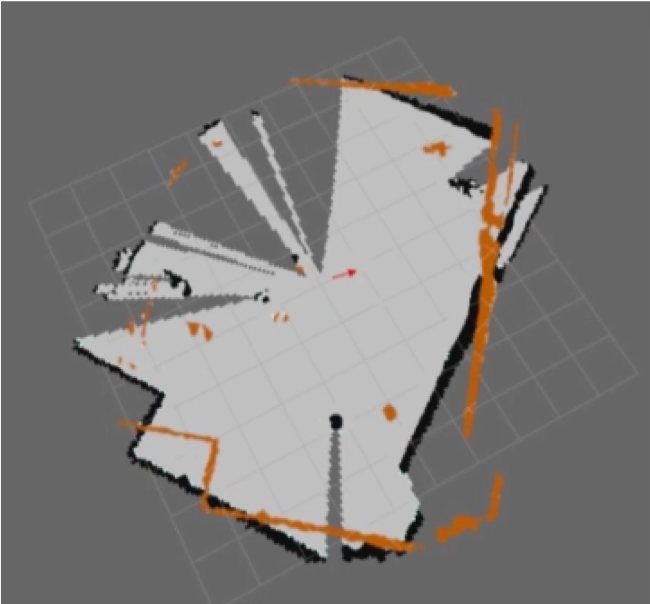
\includegraphics[width = 6cm]{Pictures/robotorientation}%
			\caption{Robot Orientation}
			\label{robot_orientation}
		\end{minipage}%
		\begin{minipage}{.5\textwidth}
			\centering
			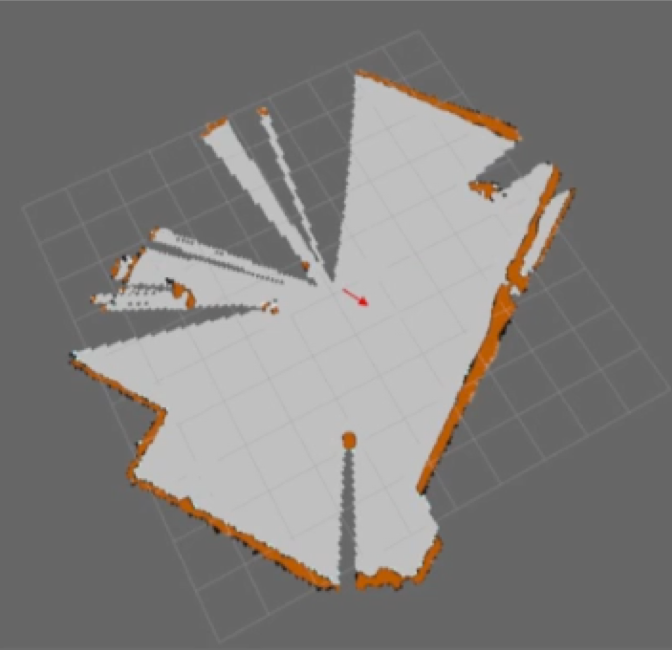
\includegraphics[width = 6cm]{Pictures/correctionwithglobalmap}%
			\caption{Correction with global map}
			\label{correction_with_globalmap}
		\end{minipage}
	\end{figure}\\
 	Initially the robot assumes a position as shown in fig.\ref{robot_orientation}, and as it moves it begins to re-correct it's estimated orientation using the static obstacle with the global map as a reference as shown in fig. \ref{correction_with_globalmap}. 
\end{itemize}
\subsubsection*{Pro and con}
Based on the research made, two tables with advantages and disadvantages of the two Map-Based Localization systems are created.\\ 
\begin{table}[!htbp]
	\centering
	\begin{tabular}{|l|l|}
		\hline
		\multicolumn{2}{|c|}{\textbf{Using Ultrasonic Sensor}}                                                                                                                                                                                \\ \hline
		\multicolumn{1}{|c|}{\textbf{Pro}}                                                                                & \multicolumn{1}{c|}{\textbf{Con}}                                                                            \\ \hline
		Cheap \euro3/each                                                                                                & Scan angle 30\degree                                                            \\ \hline
		Easy hardware Installation                                                                                                   & Similar landmarks cause localization error 
		\\ \hline
		\begin{tabular}[c]{@{}l@{}}Faster feedback than the previous camera\\ based localization system\end{tabular}
		& High computational effort for large plant     
		\\ \hline
		Scan range 4.5 meters
		& \begin{tabular}[c]{@{}l@{}}Robots should start at every launch from static\\ home position\end{tabular}
		\\ \hline
		\begin{tabular}[c]{@{}l@{}}Different map based localization\\ algorithms are available\end{tabular}
		& 
			                                                                                  \\ \hline
	\end{tabular}
	\caption{Pro and cons of Localization using Ultrasonic Sensor}
	\label{my-label}
\end{table}
\pagebreak

%%%%%%%%%%%%%%%%%%%%%%%%%%%%
\titleformat{\section}{\Large\bf}{\thesection}{20pt}{}
\section{Principle of localization via Radio Frequency Identification technology} \label{Sec_theor}
\subsection{Radio Frequency Identification}
After deep analysis of different localization methods the Radio Frequency Identification\cite{rfid.application}\cite{rfid.application2} was chosen due to its various advantages.
This technology involves a reader and a tag which is placed on the object to be tracked. The reader is continuously sending the radio waves, and when the tag is within the range of reader, it sends a feedback signal to the reader as shown in fig. \ref{reader_tag}. The reader can track multiple tags at the same time.
\begin{figure}[!htbp]
	\centering
	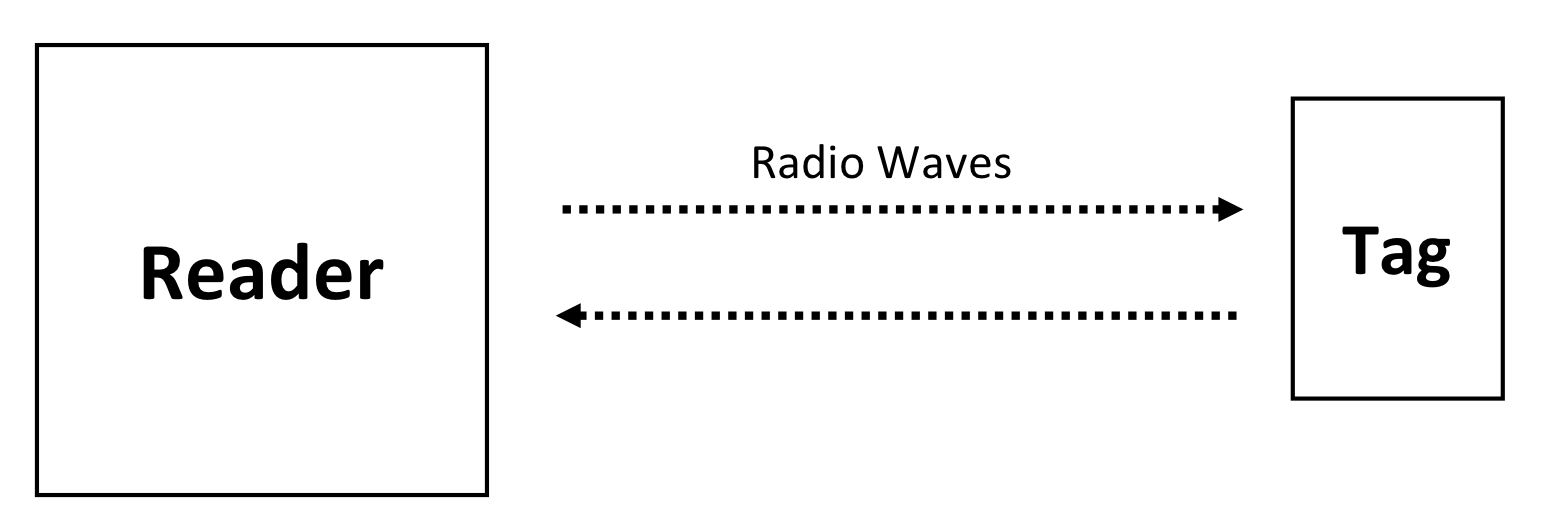
\includegraphics[width = 13cm]{Pictures/readertag}
	\caption{Reader Tag}
	\label{reader_tag}
\end{figure}
\subsubsection{RFID System}
Regarding the tags as shown in fig.\ref{rfid_system}, it can be either
\begin{itemize}
	\item Active tag which has its own power supply 
	\item Passive tag which relies on the radio waves as its source of energy that come from the reader 
	\item Semi-passive tag which has power supply, but for transmitting the feedback, it relies on the signal coming from reader
\end{itemize}
\begin{figure}[!htbp]
	\centering
	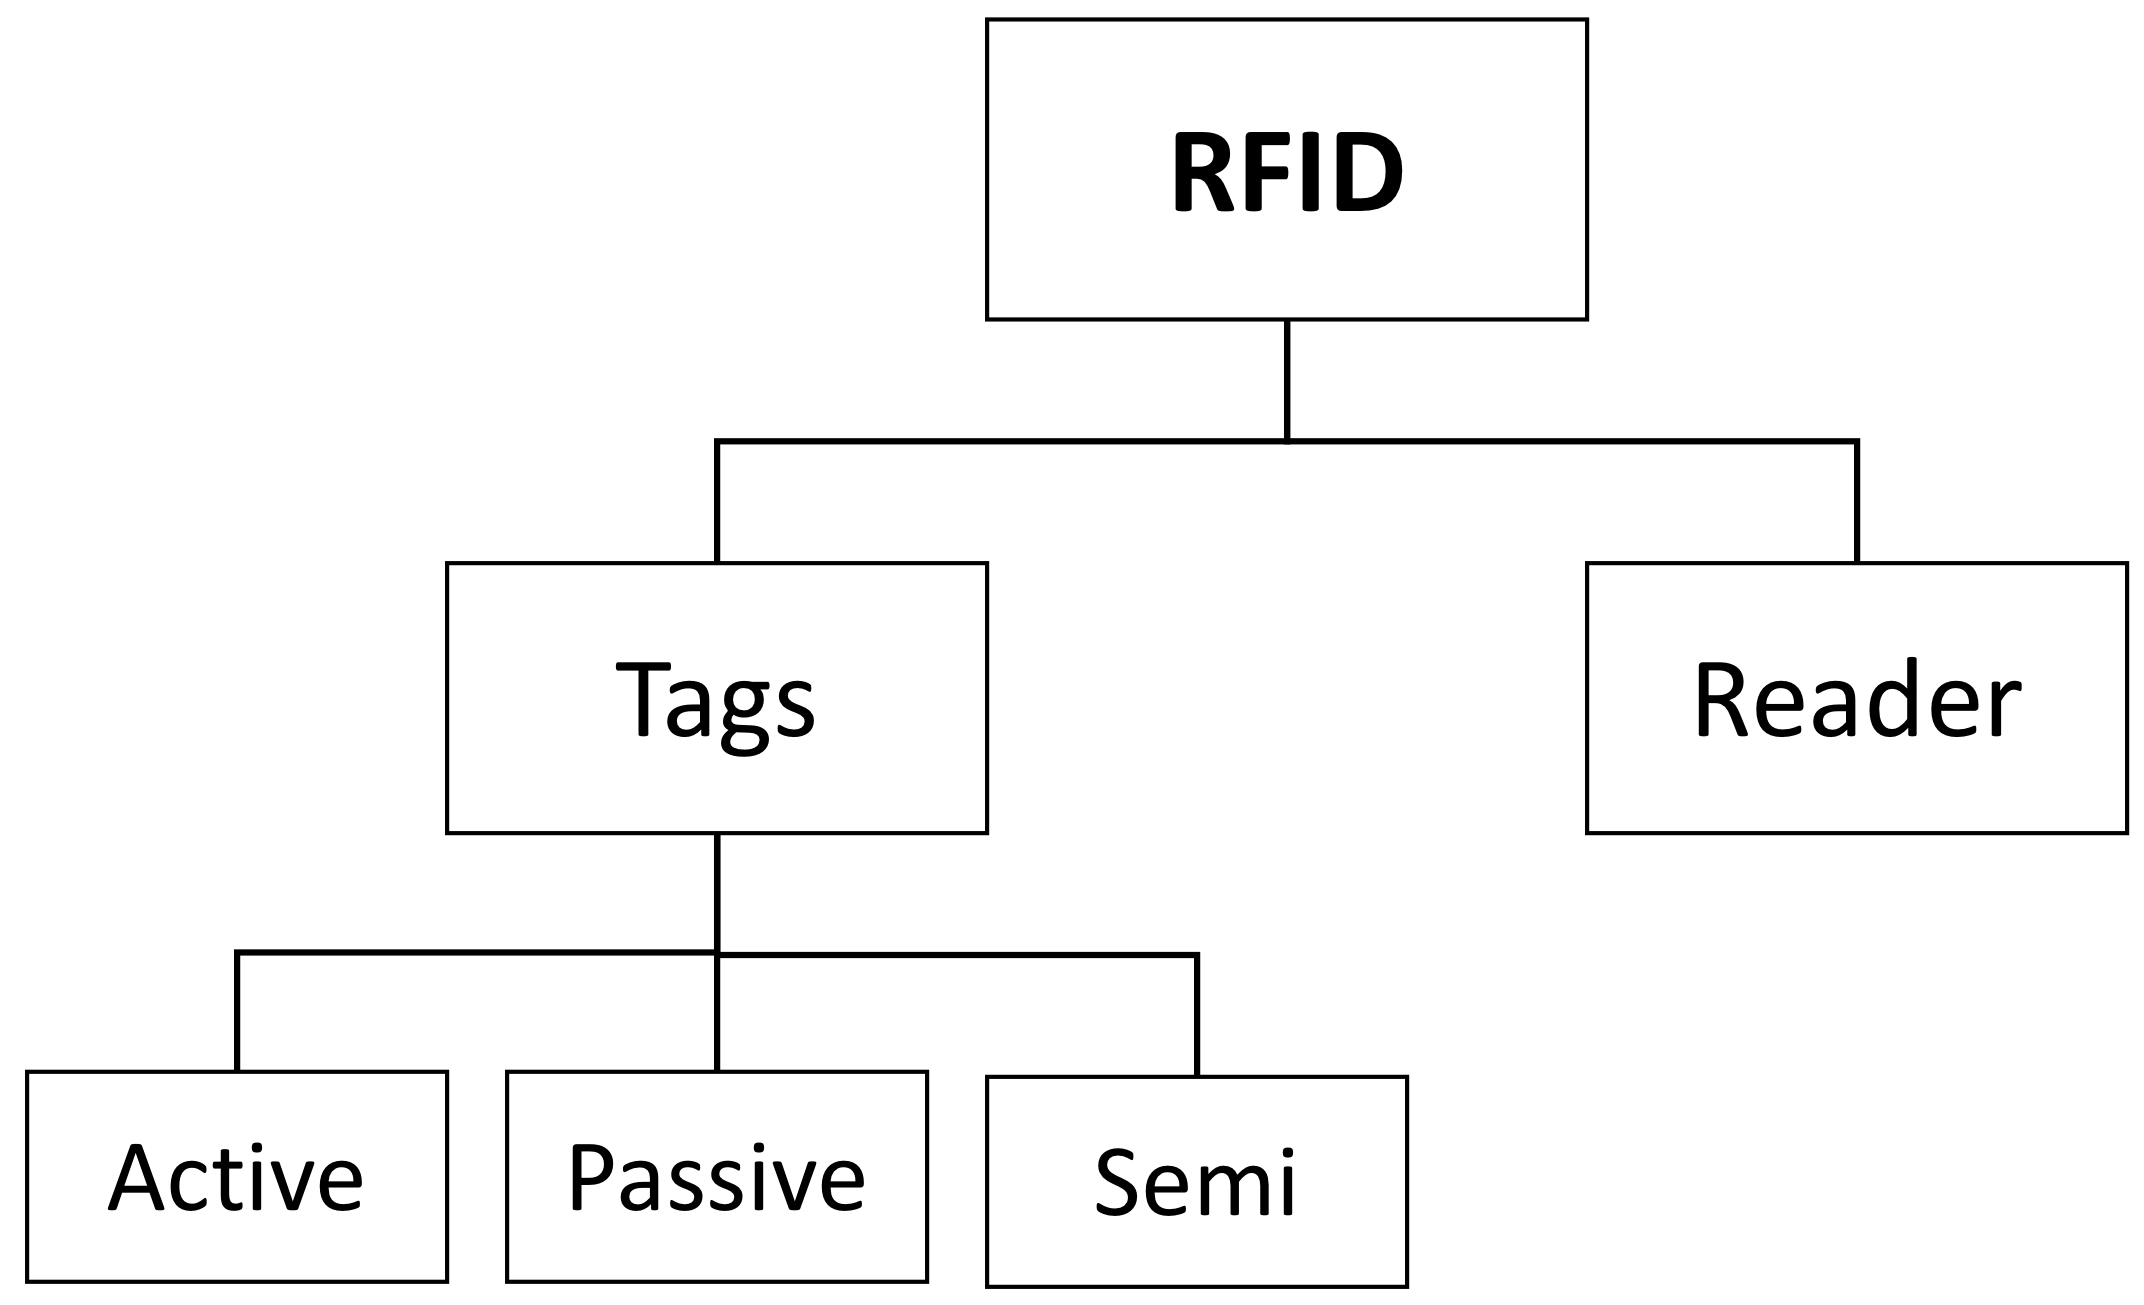
\includegraphics[width = 10cm]{Pictures/rfidsystem}
	\caption{RFID System}
	\label{rfid_system}
\end{figure}

\subsubsection{Working Principle}

The RFID consists of three main parts:
\begin{itemize}
		\item A Generator which generates the radio waves
		\item A signal detector which receives the feedback from the tag
		\item Micro-controller which processes the information from the generator and the detector\\
		\\
	\end{itemize}
The tags consists of:
\begin{itemize}
	\item Transponder: that receives radio waves and sends the feedback
	\item Rectifier Circuit: which stores the energy coming from the wave across the capacitor, and this energy is used as a power supply for the controller as well as the memory
\end{itemize}

\begin{figure}[!htbp]
	\centering
	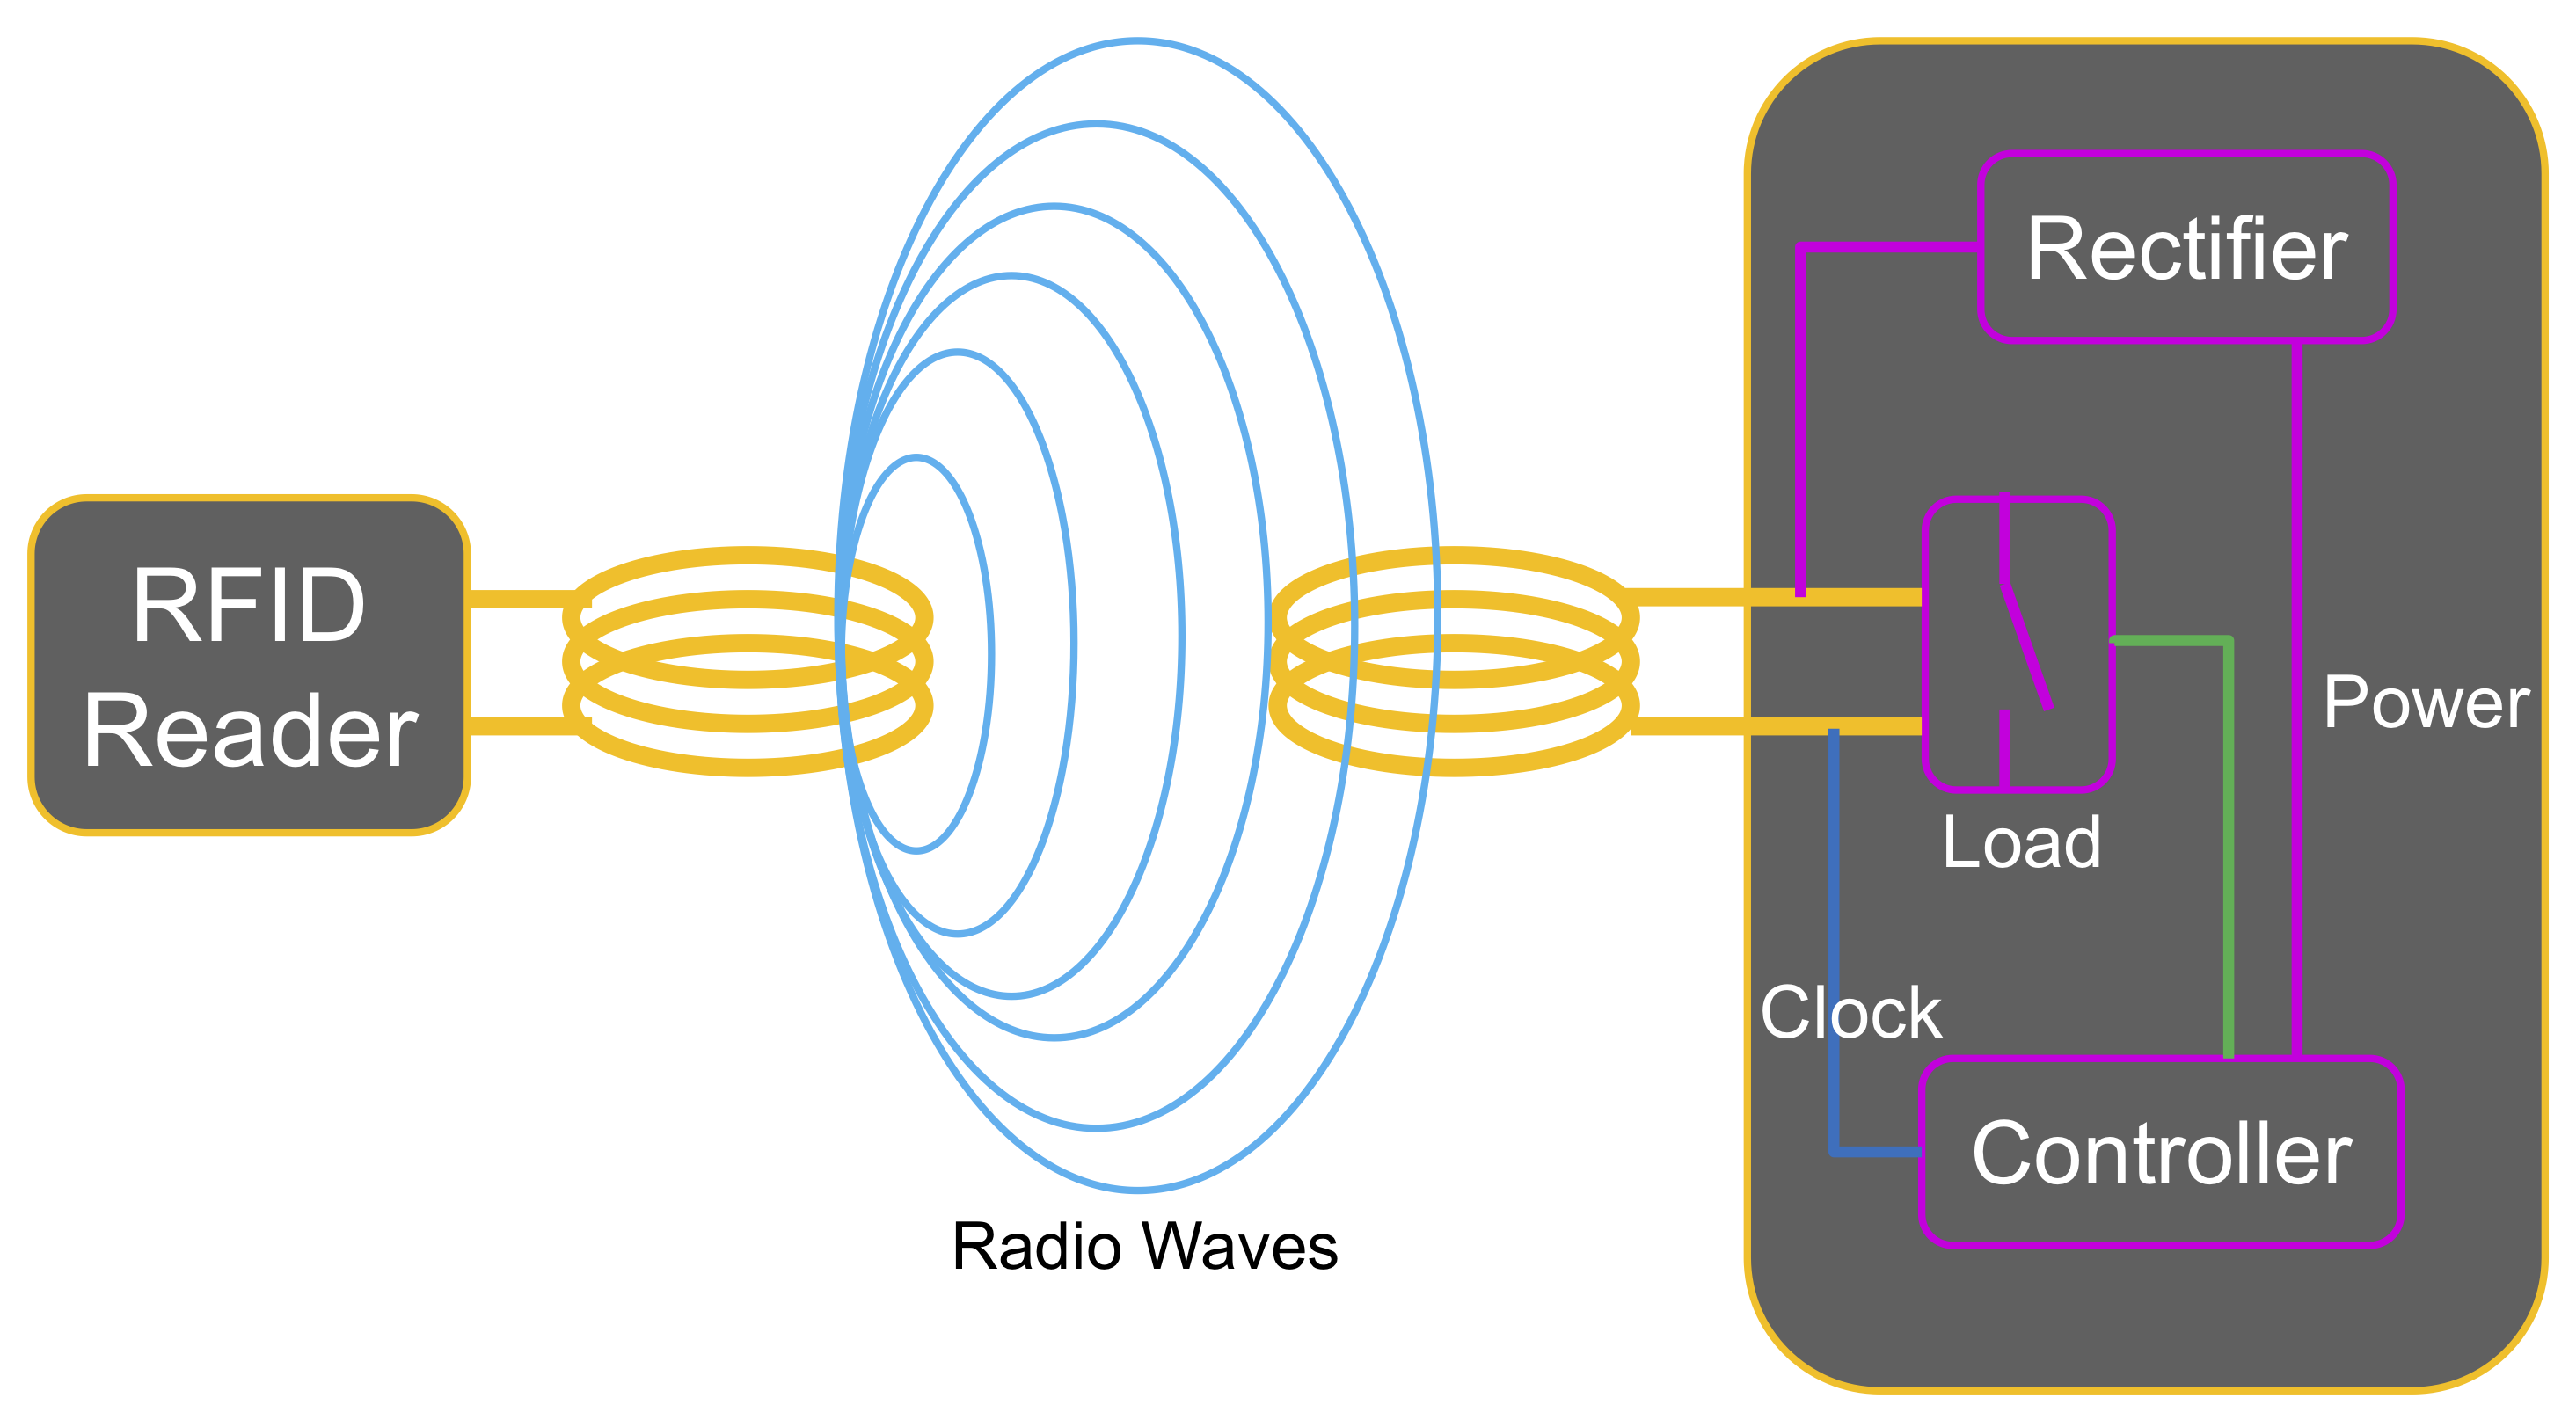
\includegraphics[width = 13cm]{Pictures/rfidtotag}
	\caption{Inductive Coupling}
	\label{rfid_to_tag}
\end{figure}
The whole process of sending the information between the tag and the reader is based on principle of "Inductive coupling" as shown in fig. \ref{rfid_to_tag}.
The reader is continuously sending radio waves with particular frequency. In this case, the reader and tag should be within the range of the frequency. The field which is generated by the reader is used coupling antenna of the tag, and due to the mutual coupling, the voltage is induced across the coil of the tag. The voltage is rectified and used as power supply for the controller and derive synchronization clock for the controller.\\
When the load circuit is connected to the coil, the current starts flowing through it. Therefore, when the load is switched on and off , the current will be turned on and off respectively leading to the induction of particular voltage in the reader. This method of switching the load is called load modulation. Thus, with the help of load modulation with respect to the data stored in the tag, the value of the induced voltage can be modified. Which leads to the generation of modulation on carrier frequency, thereby sending the data to the reader.\\
\subsection[Trilateration]{Trilateration\footnote{Stephan}}
Trilateration is a method to compute the intersection point of three circles/spheres. For this, it is necessary to know the three center of the circles/spheres plus their corresponding radii. The basic idea to estimate the intersection point is to use the mathematical description of a sphere:
\begin{align}\label{Eq_Tri}
r^2 = (x-x_1)^2 + (y-y_1)^2 + (z-z_1)^2  
\end{align} 
where ($P_n=(x_n,y_n,z_n$)) is the center of the sphere \cite{Cotera.2016}. A few assumption can be made to simplify (\ref{Eq_Tri}) for the 2D indoor localization on a floor. First of all, the z-component of all spheres can be neglected. Another assumption is that we define the origin of the first circle as the center of the coordinate system, the second along the x-axis with an distance (d) and the third shifted in x- (i) and y-direction (j), which is illustrated in following fig.\\ 
\begin{figure}[!htbp]
 \centering
 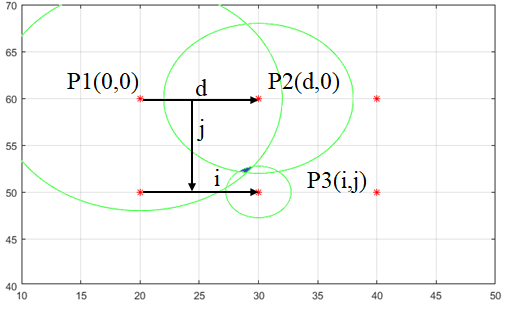
\includegraphics[width = 13cm]{Pictures/Trilateration_1}
 \caption{Overview Trilateration}
 \label{Tri_1}
 \end{figure}\\ 
With known positions of the center of the circles d, i and j can be computed in the following way\cite{Cotera.2016}:
\begin{align}
d = |P_2 - P_1| \\ 
e_x = \dfrac{1}{d}(P_2 - P_1) \\
a_x = P_3 - P_1 \\
i = e_x \cdot a_x \\
a_y = (P_3 - P_1) - i * e_x \\
e_y = \dfrac{a_y}{|a_y|} \\
j = e_y \cdot a_x
\end{align}
It has to be notice that $P_1$,$P_2$  and $P_3$ are 2D vectors, which represents the x- and y-coordinate of the points.\\ 
After knowing these values, the relative distance from the origin of the coordinate system can be computed with the help of (\ref{Eq_Tri}) and the center of the circles $P_1$(0,0), $P_2$(0,d) and $P_3$(i,j) as follows:
\begin{align}
x_t = \dfrac{r_1^2 - r_2^2 + d^2}{2*d} \\
y_t = \dfrac{r_1^2 - r_3^2 + i^2 + j^2}{2*j} - i* \bigg(\dfrac{x_t}{j}\bigg) 
\end{align}
The absolute position of the intersection point is computed in following way:
\begin{align}
P = P_1 + e_x * x_t + e_y * y_t 
\end{align}
It can be seen, that those equations are using the first two points plus radii to estimate the x-coordinate and first and third point plus the estimated x-coordinate to estimate the y-coordinate.\\ 


%%%%%%%%%%%%%%%%%%%%%%%%%%%%
\titleformat{\section}{\Large\bf}{\thesection}{20pt}{}
\section{Hardware}\label{Sec_Har}

\subsection{RFID reader and antenna}
The RFID reader from KTS Systeme (see fig.\ref{Reader}) is a HF Modul (frequency around 13.56 MHz). It contains a full-fledged microcontroller with a high-performance RFID transceiver Integrated Circuit (IC). It has a 1.27 mm pitch pin-headers for Through Hole Technology (THT) mounting. The connection to an external antenna can be realized via a single ended 50 $\Omega$ connection or via pin header U.FL. jack, which was used in this project. \\
\begin{figure}[!htbp]
\centering
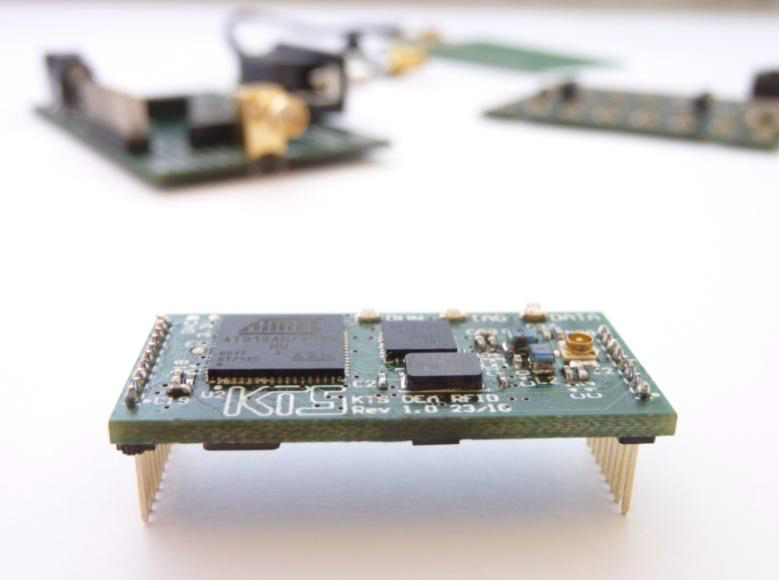
\includegraphics[width = 8cm]{Pictures/Reader}
\caption{RFID reader KTS Systeme RFIDM1356-001}
\label{Reader}
\end{figure}\\
The communication to other devices is realized via a Universal Asynchronous Receiver-Transmitter (UART) compatible serial interface via pin 6 (RX) and 7 (TX). The power supply is a 5 V DC connection via pin 1 (VCC) and pin 10 (GND). The reader is standardized to ISO 15693 and ISO14443A/B and has the overall dimensions 36 x 16 x 4 mm [LxWxH]\cite{KTSSysteme.2017}.\\
The reader has three LEDs:
\begin{itemize}
	\item Green: Run - Lights when reader receives power
	\item Yellow: Tag - Lights when a tag is detected
	\item Red: Data - Lights when data transfer to or from a tag
\end{itemize}
To configure the reader, KTS Systeme also provides a software (Tag2Image) for free. The reader was configured to scan the environment in an automatic anti collision mode (AT+Scan=AC,RSSI). Anti collision means that multiple tags can be detected at the same time and is highly important in this project. The output of the scan is a continuous information of the Identification (ID) and the Received Signal Strength Indicator (RSSI) of the detected tags. For example: SCAN:+UID=E00402000018313E,+RSSI=7/6 means that the tag with the ID (in hex) E00402000018313E was detected with a RSSI of 7/6. For the RSSI is the first number the value for the main and the second for the auxiliary receiver channel. In this project only the first number of the RSSI was used, because they are almost the same. The RSSI is an integer value from 0 to 7 and gives an information about the distance between the antenna and the detected tag. 0 stands for the maximum reading range which was mentioned to be around 15 cm. A detailed relation was obtained through experiments during the project and will be explained later in this report. An AT Command Reference Guide is also available on http://rfid.kts-systeme.de/downloads/.\\
\\
The antenna (fig. \ref{Antenna}) is a HF PCB Antenne (PCBA1356$\_$8) also from the company KTS Systeme. It has a dimension of 80 x 80 mm. The connection to the reader is realized by a SMA jack and has a self-impedance of 50$\Omega$. The antenna is designed for passive tags in a frequency range around 13.56 MHz and has a maximum power of 1W. \\
\begin{figure}[!htbp]
\centering
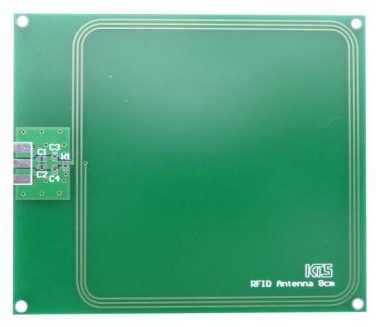
\includegraphics[width = 6cm]{Pictures/Antenna}
\caption{RFID Antenna KTS Systeme PCBA1356$\_$8}
\label{Antenna}
\end{figure}\\
The antenna and the reader are connected with a SMA to U.FL. adapter cable.\\

\subsection{RFID tag}
The tag used in the prototype is of paper type (see fig.\ref{tag}) due to its added advantages as follows:
\begin{itemize}
	\item The tags are cheap costing 18 cents each.
	\item It doesn't require power supply.
	\item The tags are compact.
	\item The implementation in the time of plant extension is simple.
\end{itemize}
\begin{figure}[!htbp]
	\centering
	\begin{minipage}{.5\textwidth}
		\centering
		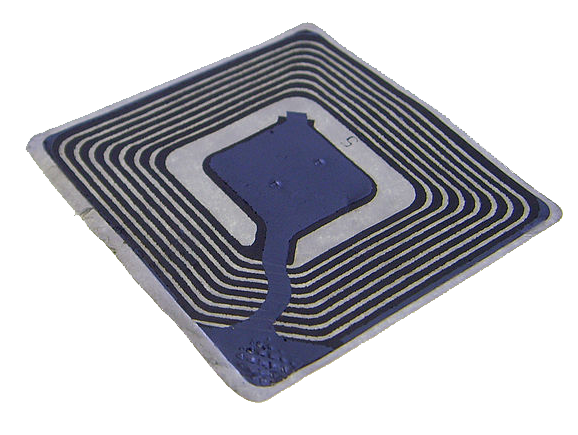
\includegraphics[width = 6cm]{Pictures/tag}%
		\caption[The ListOfFigures caption]{Paper Tag \footnotemark[1]}
		\label{tag}
	\end{minipage}%
	\begin{minipage}{.5\textwidth}
		\centering
		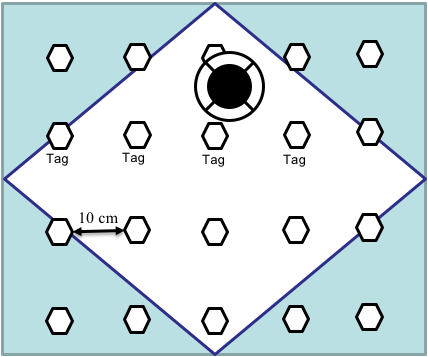
\includegraphics[width = 6cm]{Pictures/tagsfloor}%
		\caption{Tags on the plant floor}
		\label{tags_floor}
	\end{minipage}
\end{figure}
It's working principle is based on inductive coupling with an operating frequency of 125-135 kHz and a range of 10cm. The tags are fixed on the floor at known location as shown in fig.\ref{tags_floor}.
\subsection{Wifi Module}
The WiFi module used is from WEMOS Co.\cite{wemosd1mini}.It is a mini WiFi board with 4MB flash based on ESP-8266 which is a WiFi microchip with full IP/TCP stack and micro-controller (see fig.\ref{wemos}).
\footnotetext[1]{Source: \url {www.kurzweilai.net/scientists-print-cheap-rfid-tags-on-paper}}
\footnotetext[2]{Source:\url{ www.github.com/mcauser/Fritzing-Part-WeMos-D1-Mini}}
\begin{figure}[!htbp]
	\centering
	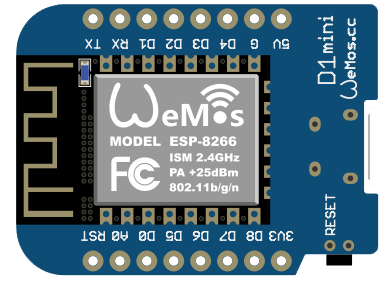
\includegraphics[width = 5cm]{Pictures/wemos}
	\caption[The ListOfFigures caption]{WeMos D1 Mini WiFi Module \footnotemark[2]}
	\label{wemos}
\end{figure}
\\
The WeMos module has the following features:
\begin{itemize}
	\item 32-bit RISC microprocessor core running at 80 MHz
	\item External QSPI flash of 4 MB
	\item IEEE 802.11 b/g/n Wi-Fi
	\item 16 GPIO pins
	\item UART on dedicated pins, plus a transmit-only UART can be enabled on GPIO2
	\item 10-bit ADC and \(I^2C\) (software implementation)
\end{itemize}
\subsection{Hardware Setup}
\begin{figure}[!htb]
	\centering
	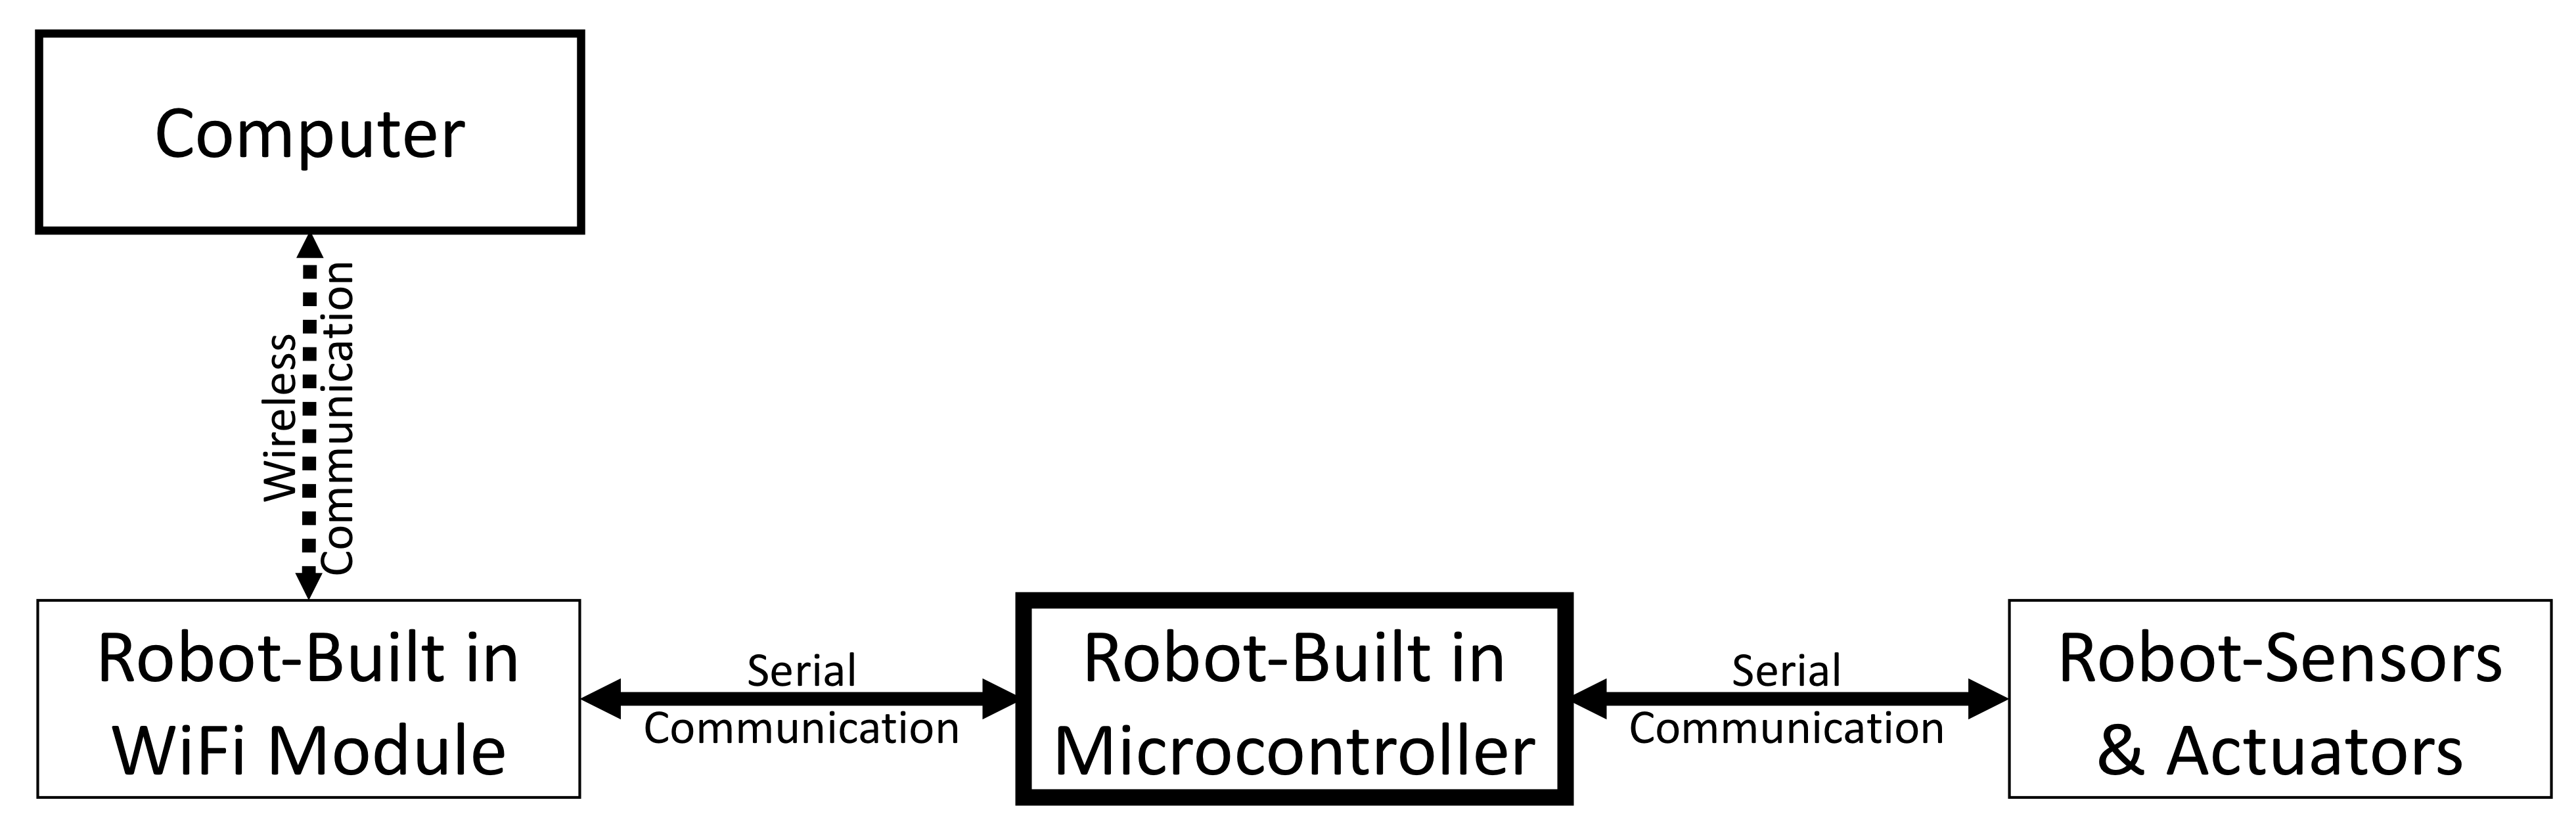
\includegraphics[width = 13cm]{Pictures/roboschematic}
	\caption{Robot Hardware Schematic}
	\label{robo_schematic}
\end{figure}
The built-in Micro-controller on the robot receives the sensor data and sends commands to the actuators via serial communication using its first UART pins. (TX/RX) is the process of sending and propagating an analogue or digital information signal over a physical point-to-point wired connection. It uses its second UART pins to communicate with the built-in WiFi Module. The built-in WiFi Module sends the received sensors data to the Computer and sends the received commands from the computer to the robot micro-controller via Wireless communication (see fig.\ref{robo_schematic}).
\begin{figure}[!htb]
	\centering
	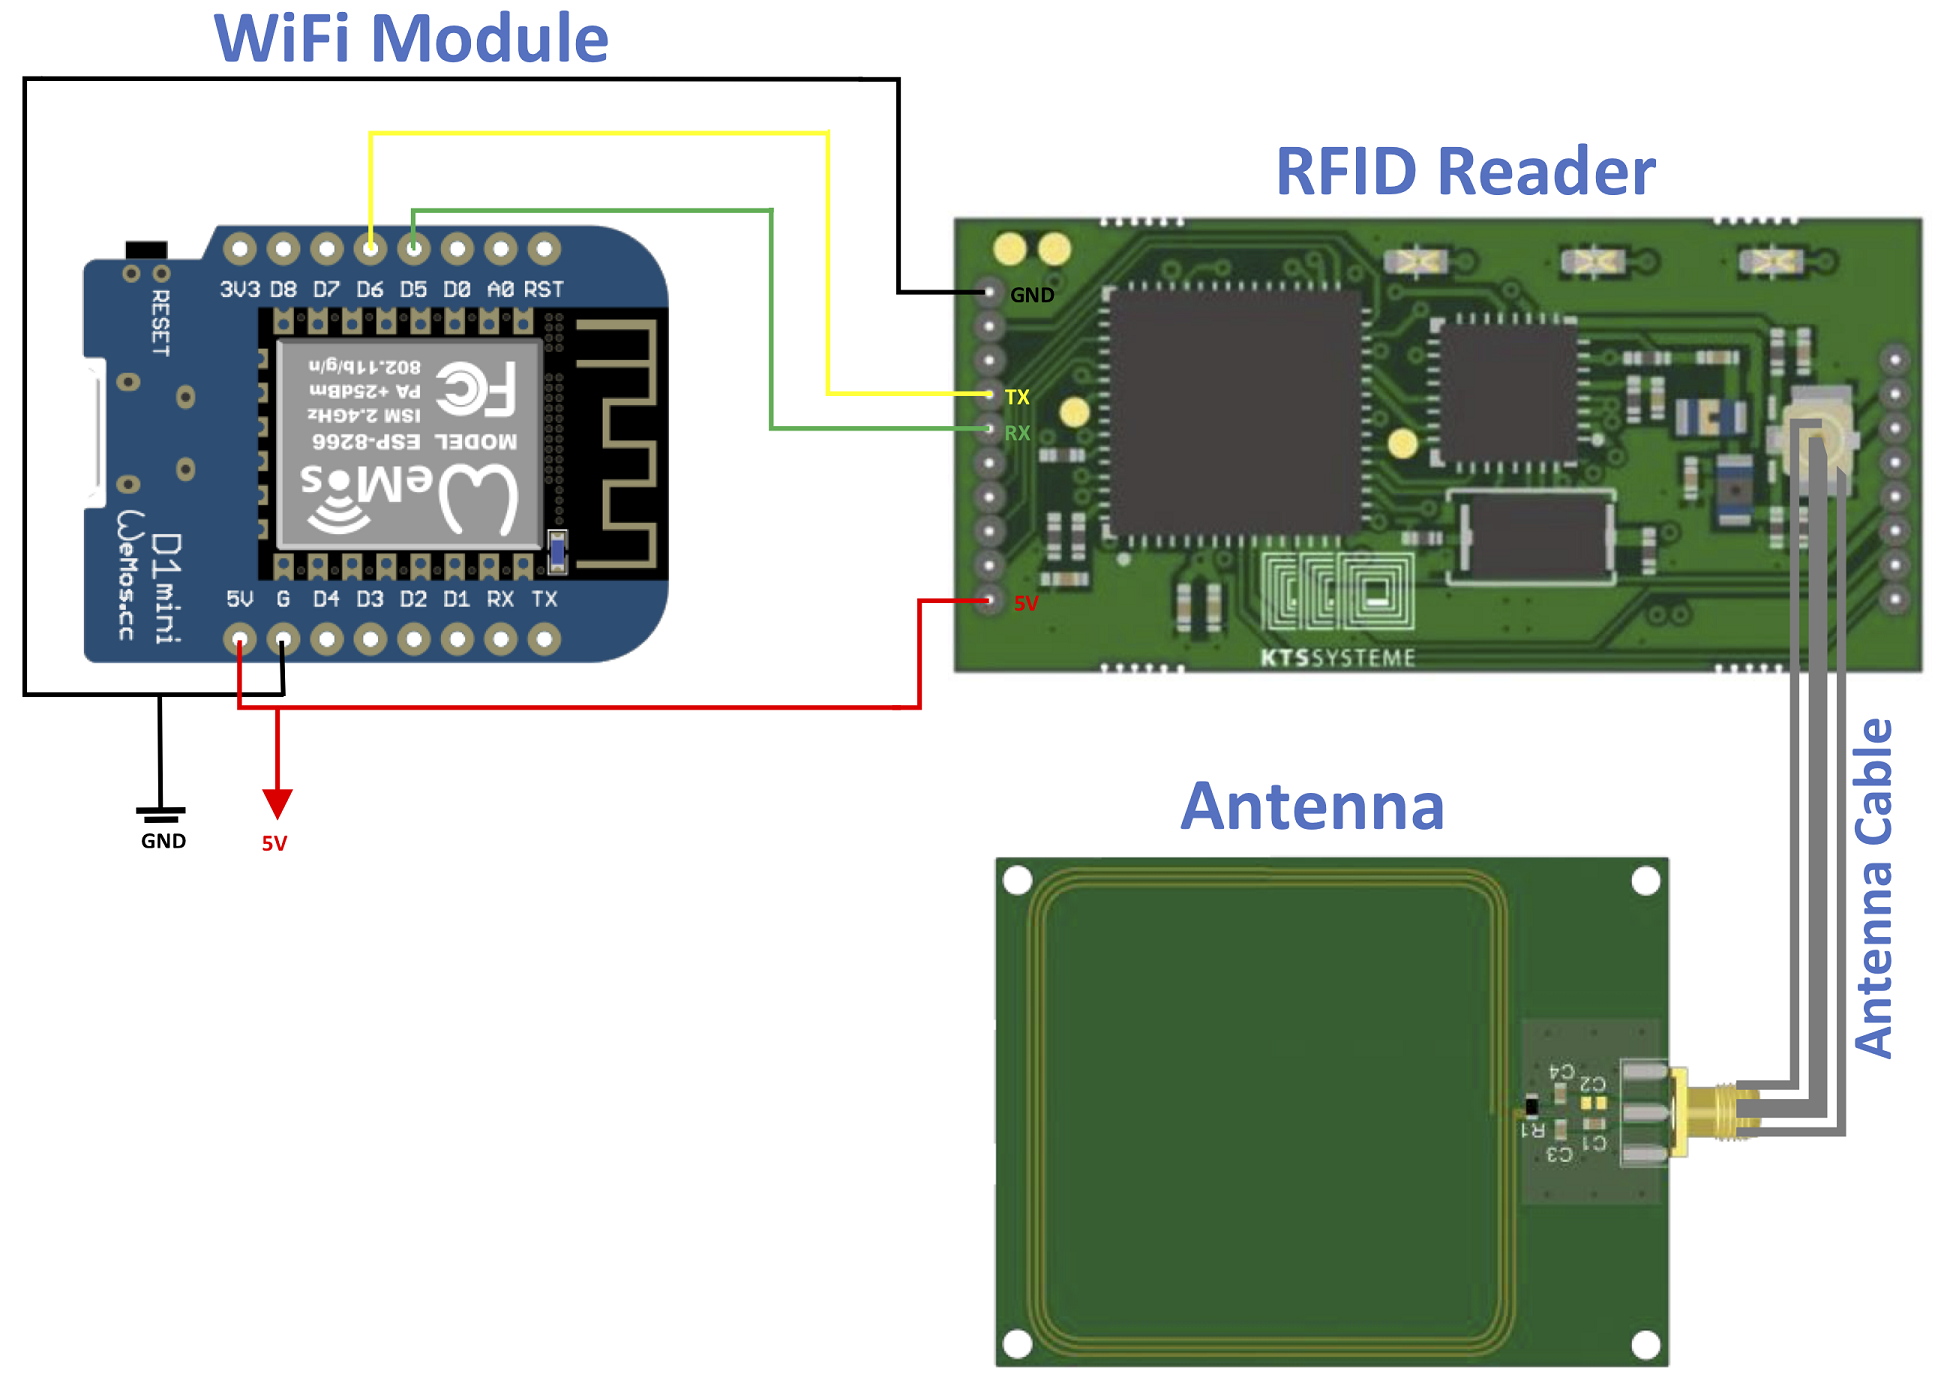
\includegraphics[width = 11cm]{Pictures/hwschematic}
	\caption{Hardware Schematic}
	\label{hw_schematic}
\end{figure}
Due to its less complexity, more flexibility and that the robot's in built micro-controller UART pins are in use, a new communication setup was developed for the RFID reader to send the data from the robot to the computer in parallel to the robot hardware setup. As shown in fig.\ref{hw_schematic}) the RFID reader is connected directly to the built-in micro-controller of the WeMos WiFi Module via serial communication sending it the tags IDs. The WeMos WiFi Module sends the received data through the network. The RFID reader is connected to the antenna which sends and receives the radio waves via SMA antenna cable.\\
The RFID reader as well as WeMos Module are placed on the top of the robot while the Antenna is fixed to the robot base such that the radio waves would be in direct contact with the tags on the floor.
\begin{figure}[!htbp]
	\centering
	\begin{minipage}{.5\textwidth}
		\centering
		\includegraphics[width = 5cm]{Pictures/rfidonrobot}%
		\caption{Top of the Robot}
		\label{rfid_on_robot}
	\end{minipage}%
	\begin{minipage}{.5\textwidth}
		\centering
		\includegraphics[width = 5cm]{Pictures/antennaonrobot}%
		\caption{Base of the Robot}
		\label{antenna_on_robot}
	\end{minipage}
\end{figure}

%%%%%%%%%%%%%%%%%%%%%%%%%%%%
\titleformat{\section}{\Large\bf}{\thesection}{20pt}{}
\section{Simulation} \label{Sec_Sim}
The simulation was carried out to answer important design questions before the real implementation phase. Furthermore artificial RFID reader data was created to test and simulate the algorithm, which will be explained in chapter \ref{Sec_Imp}. \\
To answer the design questions, the simulation has the following parameter (Appendix \ref{Sec_AppA} Line 1-50):\begin{itemize}
	\item the size of the simulation space
	\item distance between the tags
	\item distance between the first/last row/column of tags and the boarder of the simulation space
	\item diameter of the robot
	\item position of the antenna related to the origin of the robot
	\item the relation between RSSI and the distance antenna and tag
	\item initial start position and orientation
	\item difference between the measurement points of the initialization procedure
	\item optional: cycle time and speed of the robot (for another procedure)
	\item logging parameter (look of the logged text file)
\end{itemize}	
Foregone tests lead to a distance between the tags of 10 cm. This was founded on the fact that in this case at least four tags are detected at the same time (maximum reading range of 14 cm). In this case around 121 tags are needed for every square meter. This is a realistic number of tags for a small plant size, because it will lead to around 800 tags for the hole plant. \\

\subsection{Emulator}
To create artificial RFID reader data, the emulator is able to write all detected tags together with information about the measuring point into a text file. During the initialization procedure, which was the main focus in this project, the robot turns around 360 $^\circ$ and makes measurements every 45$^\circ$. \\
The emulator computes the distance from the center of the antenna to the neighbouring tags at each measurement point. If a tag is closer than the maximal reading distance, the emulator writes the detected ID of the tag together with its RSSI into the text file. \\
The RSSI is, as expalined earlier, an integer value from 0...7. 0 defines in this case a distance from 14 to around 10 cm from the antenna to the tag. In the first version of the emulator the RSSI mentioned a consistent increasing of the RSSI while the distance between the tags and the antenna gets smaller \cite{ChristofRohrigDanielHessandFrankKunemund.}. \\
During own measurements it has been found out that this relation is inconsistent. Therefore the second version of the emulator was updated and creates more realistic data.\\

\subsection{RSSI Measurements with real hardware}\label{Sec_Sim_Mea}
The relation of the RSSI is not just related to the distance between the antenna and the tag. It also depends on the orientation of the plain of the antenna and the tag. The tests with the real hardware was performed in a setup where the tags were placed on a floor and the antenna was parallel to the floor at a hight of 1.5 cm. The reason for this was the fact that the antenna should be placed directly under the robot. Tbl. \ref{RSSI_Dis_data} and fig. \ref{RSSI_Dis} present the results of the measurements.\\
\begin{table}[!htbp]
\centering
\begin{tabular}{|c|c|c|c|c|c|c|c|c|}
\hline
\begin{tabular}[c]{@{}c@{}}RSSI \\ (Received Signal Strength Indicator) \end{tabular}  & 0/0 & 1/1 & 2/2 & 3/3 & 4/4 & 5/5 & 6/6 & 7/7 \\ \hline
\begin{tabular}[c]{@{}c@{}}Maximal distance \\ antenna to tag [cm]\end{tabular} & 14  & 9.8 & 9   & 8   & 7   & 6   & 3.5 & 2.8 \\ \hline
\begin{tabular}[c]{@{}c@{}}Middle distance\\ antenna to tag [cm]\end{tabular}   & 5   & 5.1 & 5.3 & 5.5 & 5.8 & 4   & -   & -   \\ \hline
\begin{tabular}[c]{@{}c@{}}Minimal distance\\ antenna to tag [cm]\end{tabular}  & -   & 4.7 & 4.5 & 4.3 & 4.2 & -   & -   & -   \\ \hline
\end{tabular}
\caption{Relation between RSSI and distance antenna to tag (data)}
\label{RSSI_Dis_data}
\end{table}\\
\begin{figure}[!htbp]
\centering
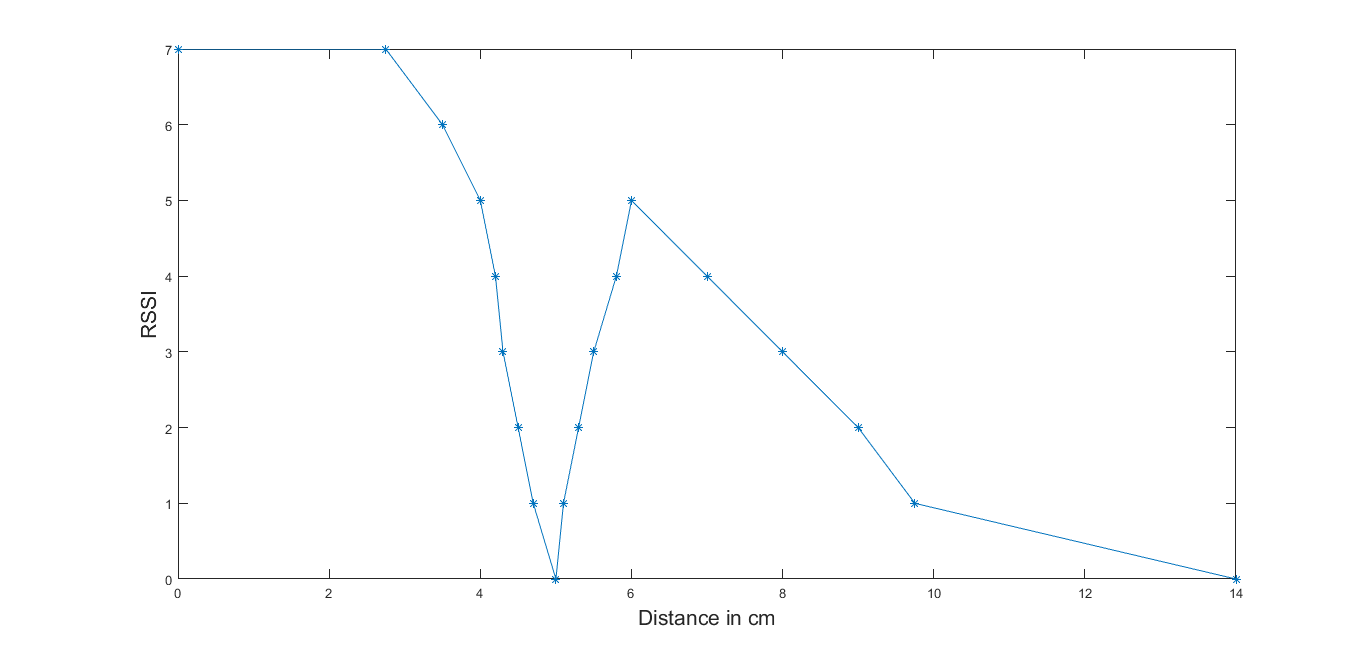
\includegraphics[width = 14cm]{Pictures/RSSI_Distance}
\caption{Relation between RSSI and distance antenna to tag}
\label{RSSI_Dis}
\end{figure}\\
Figure \ref{RSSI_Dis} demonstrates that there exists a blind spot at a distance of 5 cm where the RSSI drops to 0. The consequence is that it is not trivial to build up a relation from the RSSI back to the correct distance. \\

\subsection{Simulation with emulated data}
The idea of the final implementation is to estimate the initial position and orientation of the robot. A first version of an algorithm to solve this problem is created in matlab. The first part of these algorithm is the emulator which simulates the 360$^\circ$ turn and recordes the tag information. The second part is the solver which is also explained deeper in the chapter \ref{Sec_Imp}. \\
After observing an inconsistent behaviour of the RSSI the simulation as well as the solver were updated.\\

\subsection{Results}
The application of the emulated data on the solver indicates the following results: \\
\begin{table}[!htbp]
\centering
\begin{tabular}{|c|c|c|}
\hline
                               & \begin{tabular}[c]{@{}c@{}}Avg. accuracy position \\  (x-, \& y-direction) {[}mm{]}\end{tabular} & \begin{tabular}[c]{@{}c@{}}Avg. Accuracy \\  orientation [$^\circ$] \end{tabular} \\ \hline
Data mentioned in paper        & 2                                                                                                  & \textless{}1                                                                    \\ \hline
Own recorded data (blind spot) & 10                                                                                                 & 20                                                                              \\ \hline
\end{tabular}
\caption{Results Simulation}
\label{Res_Sim}
\end{table}\\
As can be seen from tbl. \ref{Res_Sim}, there is a sufficient good match between the estimated position and orientation of the robot for the consistent RSSI data. On the other hand the inconsistent RSSI data results in significant differences in the estimation of the position and orientation of the robot.\\
The reason for this is the higher complexity of the algorithm to first estimate the correct distances related to RSSI values and then start to estimate the position based on those distances. \\
A small error in the estimation of the position of the antenna at the first measurement point leads also to a big error in the computed orientation of the robot.

 

%%%%%%%%%%%%%%%%%%%%%%%%%%%%
\titleformat{\section}{\Large\bf}{\thesection}{20pt}{}
\section{Implementation}

\subsection{Hardware}

\subsection{Communication}

\subsection{Working}






%%%%%%%%%%%%%%%%%%%%%%%%%%%%
\titleformat{\section}{\Large\bf}{\thesection}{20pt}{}
\section{Conclusion}\label{Sec_Conc}
% https://www.wikihow.com/Write-a-Conclusion-for-a-Research-Paper
% 1. Restate the topic. You should briefly restate the topic as well as explaining why it is important.
% 2. Restate your thesis. Aside from the topic, you should also restate or rephrase your thesis statement.
% 3. Briefly summarize your main points. Essentially, you need to remind your reader what you told them in the body of the paper.
% ( 4. Add the points up. If your paper proceeds in an inductive manner and you have not fully explained the significance of your points yet, you need to do so in your conclusion. )
% ( 5. Make a call to action when appropriate. If and when needed, you can state to your readers that there is a need for further research on your paper's topic. )
% 6. Answer the “so what” question.

% Phrases: ...A key limitation of the actual setup is that
The developed localization solution was for the pipeless plant, a prototype of a chemical production plant which has a size of 3 by 4 m. In this plant the vessel will be transported by AGVs from one station to another. In the actual setup only a camera, which is installed above the plant, was used to detected the AGVs and estimate their positions. The problem with this technology is the bad detection of the LED pattern from the AGVs during bright light conditions and also the space limitation. Another big disadvantage is the big computation effort which makes the system also very slow. The main task of this project was to find an alternative tracking solution. During the project group phase differnt localization technologies were evaluated. With respect to the outcoming reseaches about triangulation, map-based-localizaion, pattern recognizion and localizaion via radio frequency identification the last RFID based localization of the AGV with passive tags as landmarks turned out to be the most promising among those four. With information of a similar project realized by the FH Dortmund a model to evaluate sample data and a localization algorithm was created in Matlab. This results of the simulation were promising and  therefore used during the decision making process about the actual hardware setup. With an demonstration board with the size of 30 cm x 30 cm the initialization procedure algorithm was implemented in which the AGV performes and 360$^\circ$ turn and estimates its position and its orientation based on measuremtns during this movement. With respect to this solutions it can be said that it is possible to assemble a reader on an AGV and detect passive tags with its antenna in a range of 14 cm. It also has been found out that an inconsistent realation between the RSSI of the detected tags and the distance based on the RSSI is not generally trivial and was only solved in a rather simple and unriliable way during the project. Based on the results computed by the initializaion prcedure, it can be concluded that it is possible to estimate the position of the AGV with an average accuracy of aroung 2.5 cm and an estimation error of the orientation of around 23$^\circ$. Compared to the former localization set up this solutions, especially with respect to the orientation error, are not perfelty satisfying and just minimal requirements are fullfilled. The received data from the RFID reader have furthermore clearly shown that the anti-collision algorithm used by the reader leads to an unknown amount of time until each and every tag in the detection area is identified. Summed up a model based demonstrator was realized which on the one hand does not improve the accuracy of the localizaion of the plant under good light conditions especially with respect to the orientation but on the other hand a promising technology for indoor localizaion with light independedcy, respectivelay cheap costs and highly scalability was found. 




%After the decision for a RFID system with passive tags as landmarks a prototype was build to verify the good solutions from the simulations. The implemented procedure was an initialization algorithm in which the the AGV makes an 360$^\circ$ turn and estimates its position and its orientation based on measurements during these turn. This project has shown that it is possible to put a reader on an AGV and detect passive tags with a reader and an antenna in an detection area of 14 cm. It has also been found out that there is inconsistent relation between the received signal strength (RSSI) of the detected tags and the distance between the tag and the reader. This leads to the fact that the estimation of the distance based on the RSSI is not trivial and was only solvable in a very simple and inaccurate way during the project. Based on the results from the initialization procedure, it can be concluded that it possible to estimate the position of the AGV with an average accuracy of around 2.5 cm and an estimation error of the orientation of around 23$^\circ$. This is not a very good results and fulfils only the minimal requirements. This project has also clearly shown that the anti-collision algorithm of the reader gives  very inefficient results and leads to an unknown amount of time until all tags in the detection area are identified. It was not possible to develop a running and faultless system, but is has been demonstrated that the system is light independent and space unlimited. Summing up all results, it can be concluded that the system is a promising technology for the indoor localizing on the small plant and gets rid of a lot of the current disadvantages. 

%%%%%%%%%%%%%%%%%%%%%%%%%%%%
\titleformat{\section}{\Large\bf}{\thesection}{20pt}{}

\section[Future Work]{Future Work\footnote{Stefan}}
After a proof-of-concept for an RFID based localizatin system has been build and a first demonstration set-up has been build the disadvantages and limitations of the prototype were evaluated. According to these results several points of improvement and extension were found and categorized into a hardware and a software section. 
\subsection{Hardware}
\begin{itemize}
\item The AGVs are feed by an included 12V battery which provides the power for all included electronical deviced. This 12V power supply is available on board and is suggeted to be used. Currently the WiFi-Module and the RFID-Reader are fed by an external powerbank since a 5V power supply is needed. In terms of one zentralized power supply a 12 V to 5 V converter can be installed and connected to the new hardware.
\item As a first set-up a demonstration area of 3 x 3 TAGs was developed. In this rather small area initializaion procedure was developed but a real time localization while a trajectory is followed by an AGV was not possible since the 30cm x 30cm was simply to small. For futrue research in terms of localizaion on a specified trajectory additional TAGs can be included to the area of operation. Since the RFID concept is highly scalable the only change that needs to be made in the algorithm is the insertion of the additional TAG into the lookup table.
\item Currently the only Robot No. 1 is the only AGV which is equipped wich the RFID technolgoy. To run the plant wich multible AGVs the remaining robots needs to be upgraded.\\
\end{itemize}
\subsection{Software}
\begin{itemize}
\item During the Initalizatin procedure a 360 degres turn is performed. The degrees are devided by the change of degree over time. But it needs to be said that this movement is highly dependend on distrubances like changing battery charge and plant underground. For the future developers it is suggested to use the encoders of the robot weels as a determination of the orientation instead the parameter time.
\item As an alternative localizatin technolgy was found several code lines in the VisualStudio can be deleted since the camera and image processing is simpls not used anymore. With a clean code an improvement of processing time will be accieved.
\item As a last point it can be said that even though a localization with RFID is now possible the results are not 100 percent realiable and the accuracy especially with respect to the orientation is not satisfing so far. As an improvement the triangulation algorithm is to be optimized and or a second RFID-Antenna is to be added under the AGV to reduce measurment errors.
\end{itemize}

%%%%%%%%%%%%%%%%%%%%%%%%%%%%
\titleformat{\section}{\Large\bf}{\thesection}{20pt}{}
\section{References}
..


%%%%%%%%%%%%%%%%%%%%%%%%%%%%
\titleformat{\section}{\Large\bf}{\thesection}{20pt}{}
\section{Appendixes}

\subsection{Emulator RFID data (Matlab)}
\lstinputlisting{code/Emulator.m}



\label{LetzteSeite} %marker letzte Seite


\end{document}

\label{LetzteSeite} %marker letzte Seite

%%%%%%%%%%%%%%%%%%%%%     EXTRA HELP    %%%%%%%%%%%%%%%%%%%%%%%%%%%%%%%%%%%%%%%%
% TO ADD A PICTURE..

% \begin{figure}[h!]
%   \includegraphics[width=\linewidth]{boat.jp g}
%   \caption{A boat.}
%   \label{fig:boat1}
% \end{figure}


% TO ADD A TABLE..

% \begin{table}[h!]
% \centering
%  \begin{tabular}{||c c c c||} 
%  \hline
%  Col1 & Col2 & Col2 & Col3 \\ [0.5ex] 
%  \hline\hline
%  1 & 6 & 87837 & 787 \\ 
%  2 & 7 & 78 & 5415 \\
%  3 & 545 & 778 & 7507 \\
%  4 & 545 & 18744 & 7560 \\
%  5 & 88 & 788 & 6344 \\ [1ex] 
%  \hline
%  \end{tabular}
%  \caption {Should be a caption}
% \end{table}

